\chapter{Phương pháp đề xuất}
\label{ch:method}

Chương này trình bày chi tiết về HSGE (Hierarchical Skill-Graph Exploration) -- chuỗi xử lý (pipeline) do nhóm nghiên cứu đề xuất nhằm chuyển đổi một website chưa được gán nhãn thành tập dữ liệu huấn luyện cho các mô hình ngôn ngữ nhỏ. Nội dung chương được cấu trúc thành các phần chính bao gồm: (1) tổng quan về pipeline và các nguyên tắc thiết kế lõi; (2) cơ chế biểu diễn đồ thị hai tầng làm nền tảng cho toàn bộ phương pháp; (3) quá trình khám phá có định hướng dựa trên đồ thị thông qua các tác vụ mức thấp (low-level task) do LLM đề xuất; (4) phương pháp phát hiện và kiểm chứng các kỹ năng (skill) có khả năng tái sử dụng; (5) cơ chế sinh các tác vụ ngữ nghĩa (\emph{semantic task}) dài hạn thông qua việc ghép chuỗi các toán tử (operator) lập kế hoạch; (6) quy trình tinh lọc quỹ đạo tương tác (trajectory) để xây dựng tập dữ liệu tinh chỉnh (fine-tuning); (7) thực hiện tinh chỉnh mô hình SLM mục tiêu; và cuối cùng là (8) một số ghi chú trong quá trình cài đặt và hiện thực hóa hệ thống.

\section{Tổng quan}
\label{sec:method-overview}

Đầu vào của hệ thống HSGE là một website đang hoạt động nhưng chưa được gán nhãn tác vụ (task), kết hợp cùng một biên khám phá (frontier) được khởi tạo từ một hoặc một vài URL hạt giống. Đầu ra là một tập dữ liệu tinh chỉnh có giám sát (SFT) bao gồm các quỹ đạo tương tác (trajectory) hướng mục tiêu, và sản phẩm cuối cùng là một mô hình ngôn ngữ nhỏ đã được tinh chỉnh (fine-tuned) trên tập dữ liệu này. Hình~\ref{fig:pipeline} thể hiện kiến trúc tổng thể của hệ thống.

\begin{figure}[htbp]
\centering
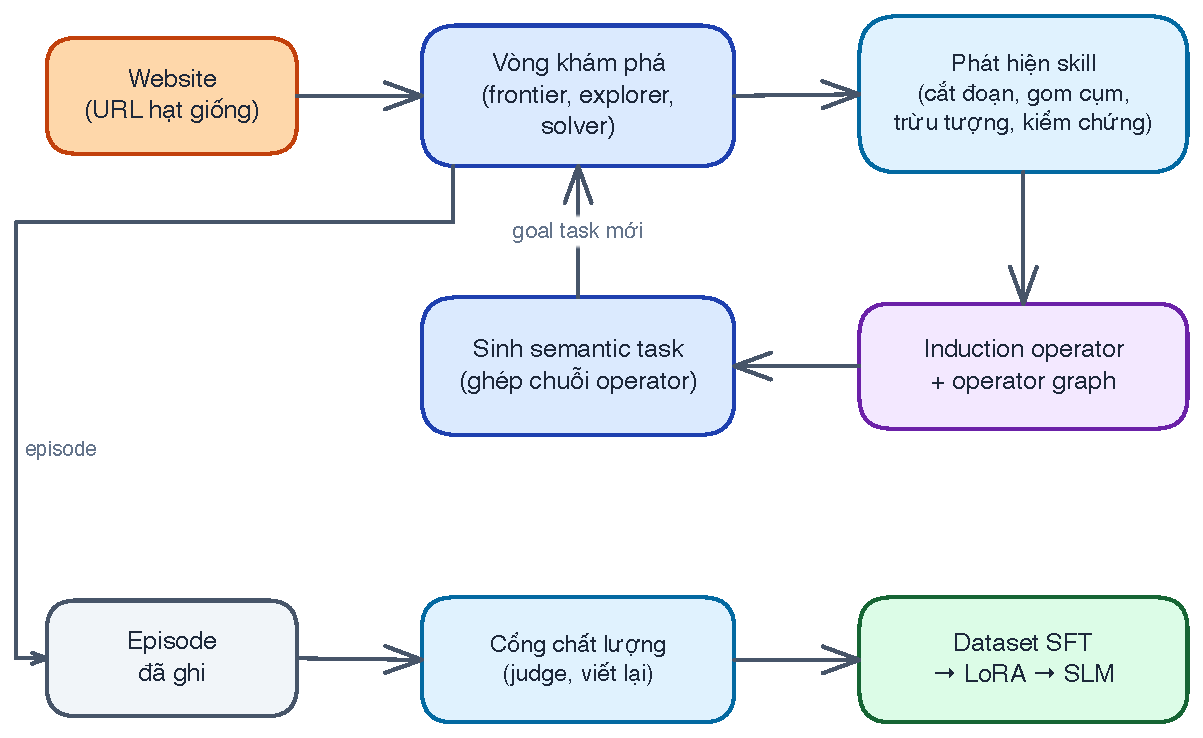
\includegraphics[width=\textwidth]{Figures/fig_pipeline.pdf}
\caption[Tổng quan pipeline HSGE]{Tổng quan chuỗi xử lý (pipeline) HSGE. Vòng lặp khám phá thực thi các tác vụ mức thấp (low-level task) do LLM đề xuất trên các trang thuộc frontier; các kỹ năng (skill) phát hiện được sẽ được nâng cấp thành các toán tử (operator) lập kế hoạch, sau đó quá trình ghép chuỗi các toán tử này sẽ tạo ra các tác vụ ngữ nghĩa (semantic task) để phản hồi ngược lại cho vòng khám phá. Mọi phiên tương tác (episode) được ghi nhận đều phải vượt qua các cổng kiểm duyệt chất lượng tự động trước khi trở thành dữ liệu huấn luyện.}
\label{fig:pipeline}
\end{figure}

Chuỗi xử lý (pipeline) này vận hành dưới dạng một vòng lặp khép kín. Tại mỗi trang được truy cập, một mô-đun khám phá (\emph{explorer}) sẽ đề xuất các tác vụ cụ thể gắn liền với nội dung của trang đó. Tiếp theo, một tác nhân giải quyết (\emph{solver} agent) sẽ thử nghiệm thực thi các tác vụ này trên trình duyệt thực, qua đó tạo ra các quỹ đạo tương tác. Thành phần phát hiện (discovery) chịu trách nhiệm phân cắt các quỹ đạo này thành từng đoạn nhỏ, gom cụm các đoạn có tính lặp lại, rồi trừu tượng hóa những cụm đã đạt độ chín thành các kỹ năng (\emph{skill}) có khả năng tái sử dụng.

Kế tiếp, hệ thống nâng cấp các skill đã qua kiểm chứng thành các toán tử (\emph{operator}) lập kế hoạch với điều kiện tiên quyết (precondition) và hiệu ứng (effect) được xác định rõ ràng. Quá trình ghép chuỗi các toán tử trên đồ thị sẽ kiến tạo nên các tác vụ mục tiêu dài hạn, được gọi là tác vụ ngữ nghĩa (\emph{semantic task}). Các tác vụ này sau đó được đưa ngược lại cho chính solver, tạo thành một vòng lặp khép kín. Mọi tác vụ được thử nghiệm, bất kể ở mức thấp hay mức ngữ nghĩa, đều được ghi nhận thành một phiên (episode). Các episode này còn phải vượt qua những cổng kiểm duyệt chất lượng tự động trước khi được biên dịch thành tập dữ liệu SFT phục vụ cho quá trình tinh chỉnh SLM mục tiêu.

Trong một lượt chạy, ba loại phiên tương tác được ghi nhận và được đánh dấu
riêng biệt, vì chúng khác nhau về điểm xuất phát chứ không chỉ về nội dung tác
vụ. Phiên \texttt{LOCAL} là một tác vụ mức thấp được giải ngay tại trang đang
xét, tức tác nhân đã đứng sẵn ở đúng nơi cần thao tác. Phiên
\texttt{UNPREFIXED} là chính tác vụ đó được giải lại một lần nữa từ trang chủ,
nên quỹ đạo bao gồm cả phần điều hướng tìm đường (Mục~\ref{sec:method-unprefixed}).
Phiên \texttt{GOAL} là một tác vụ ngữ nghĩa nhiều bước, sinh từ chuỗi operator
hoặc từ seed năng lực của website (Mục~\ref{sec:method-semantic}). Ba nhãn này
đi theo dữ liệu tới tận bước dựng tập huấn luyện, nơi chúng trở thành ba mức
độ khó của curriculum.

Quá trình thiết kế pipeline được định hướng bởi ba nguyên tắc xuyên suốt:

\begin{itemize}
  \item \textbf{P1: Kiểm chứng trước khi tái sử dụng.} Không có thông tin nào được mặc nhiên tin cậy ngay ở lần xuất hiện đầu tiên. Một skill chỉ được hệ thống thu nhận sau khi chứng minh được tính lặp lại qua các trajectory độc lập; một trạng thái tự tuyên bố thành công phải được đánh giá lại bởi một mô-đun giám khảo (judge) độc lập; và một toán tử sẽ bị loại bỏ nếu hiệu ứng của nó rỗng nghĩa.
  \item \textbf{P2: Cấu trúc đồ thị thay vì bộ nhớ phẳng.} Thay vì lưu trữ thông tin dưới dạng một tập hợp rời rạc các trang hoặc bộ nhớ phẳng, HSGE duy trì một cấu trúc đồ thị hai tầng (Mục~\ref{sec:method-graph}). Tầng thấp ghi nhận \emph{vị trí} agent đã từng đi qua; trong khi tầng cao ghi nhận những \emph{hành động} agent có thể thực hiện, cũng như cách thức các năng lực này liên kết với nhau.
  \item \textbf{P3: Hệ thống tác vụ hai tầng.} Các tác vụ mức thấp (\emph{low-level task}) do LLM đề xuất (Mục~\ref{sec:method-exploration}) đóng vai trò định hướng quá trình khám phá và cung cấp nguyên liệu thô cho việc phát hiện skill. Trong khi đó, các tác vụ ngữ nghĩa (\emph{semantic task}) (Mục~\ref{sec:method-semantic}) biểu diễn những mục tiêu nhiều bước mà không một trang web đơn lẻ nào có thể trực tiếp gợi ý. Tầng ngữ nghĩa được cấp bởi hai nguồn độc lập nhau: ghép chuỗi các năng lực đã kiểm chứng theo hướng từ dưới lên, và seed năng lực của website theo hướng từ trên xuống. Việc duy trì đồng thời hai nguồn là một quyết định thiết kế có chủ đích, xuất phát từ thực nghiệm: nguồn từ dưới lên chỉ hoạt động khi đồ thị toán tử đã có cạnh, một điều kiện thưa hơn dự kiến rất nhiều (Mục~\ref{sec:disc-operators}).
\end{itemize}

\section{Biểu diễn đồ thị hai tầng}
\label{sec:method-graph}

Hình~\ref{fig:twolevel} minh họa cấu trúc biểu diễn được đề xuất trong mục này. Tầng thấp ghi lại quá trình tương tác thực tế: các trang web mà agent đã truy cập và những hành động nó thực hiện giữa các trang đó. Tầng cao lưu trữ các năng lực có khả năng tái sử dụng: các kỹ năng (skill) được trừu tượng hóa từ quá trình tương tác, cùng với các cạnh toán tử (operator) chỉ ra cách thức chúng có thể được ghép nối với nhau.

\begin{figure}[htbp]
\centering
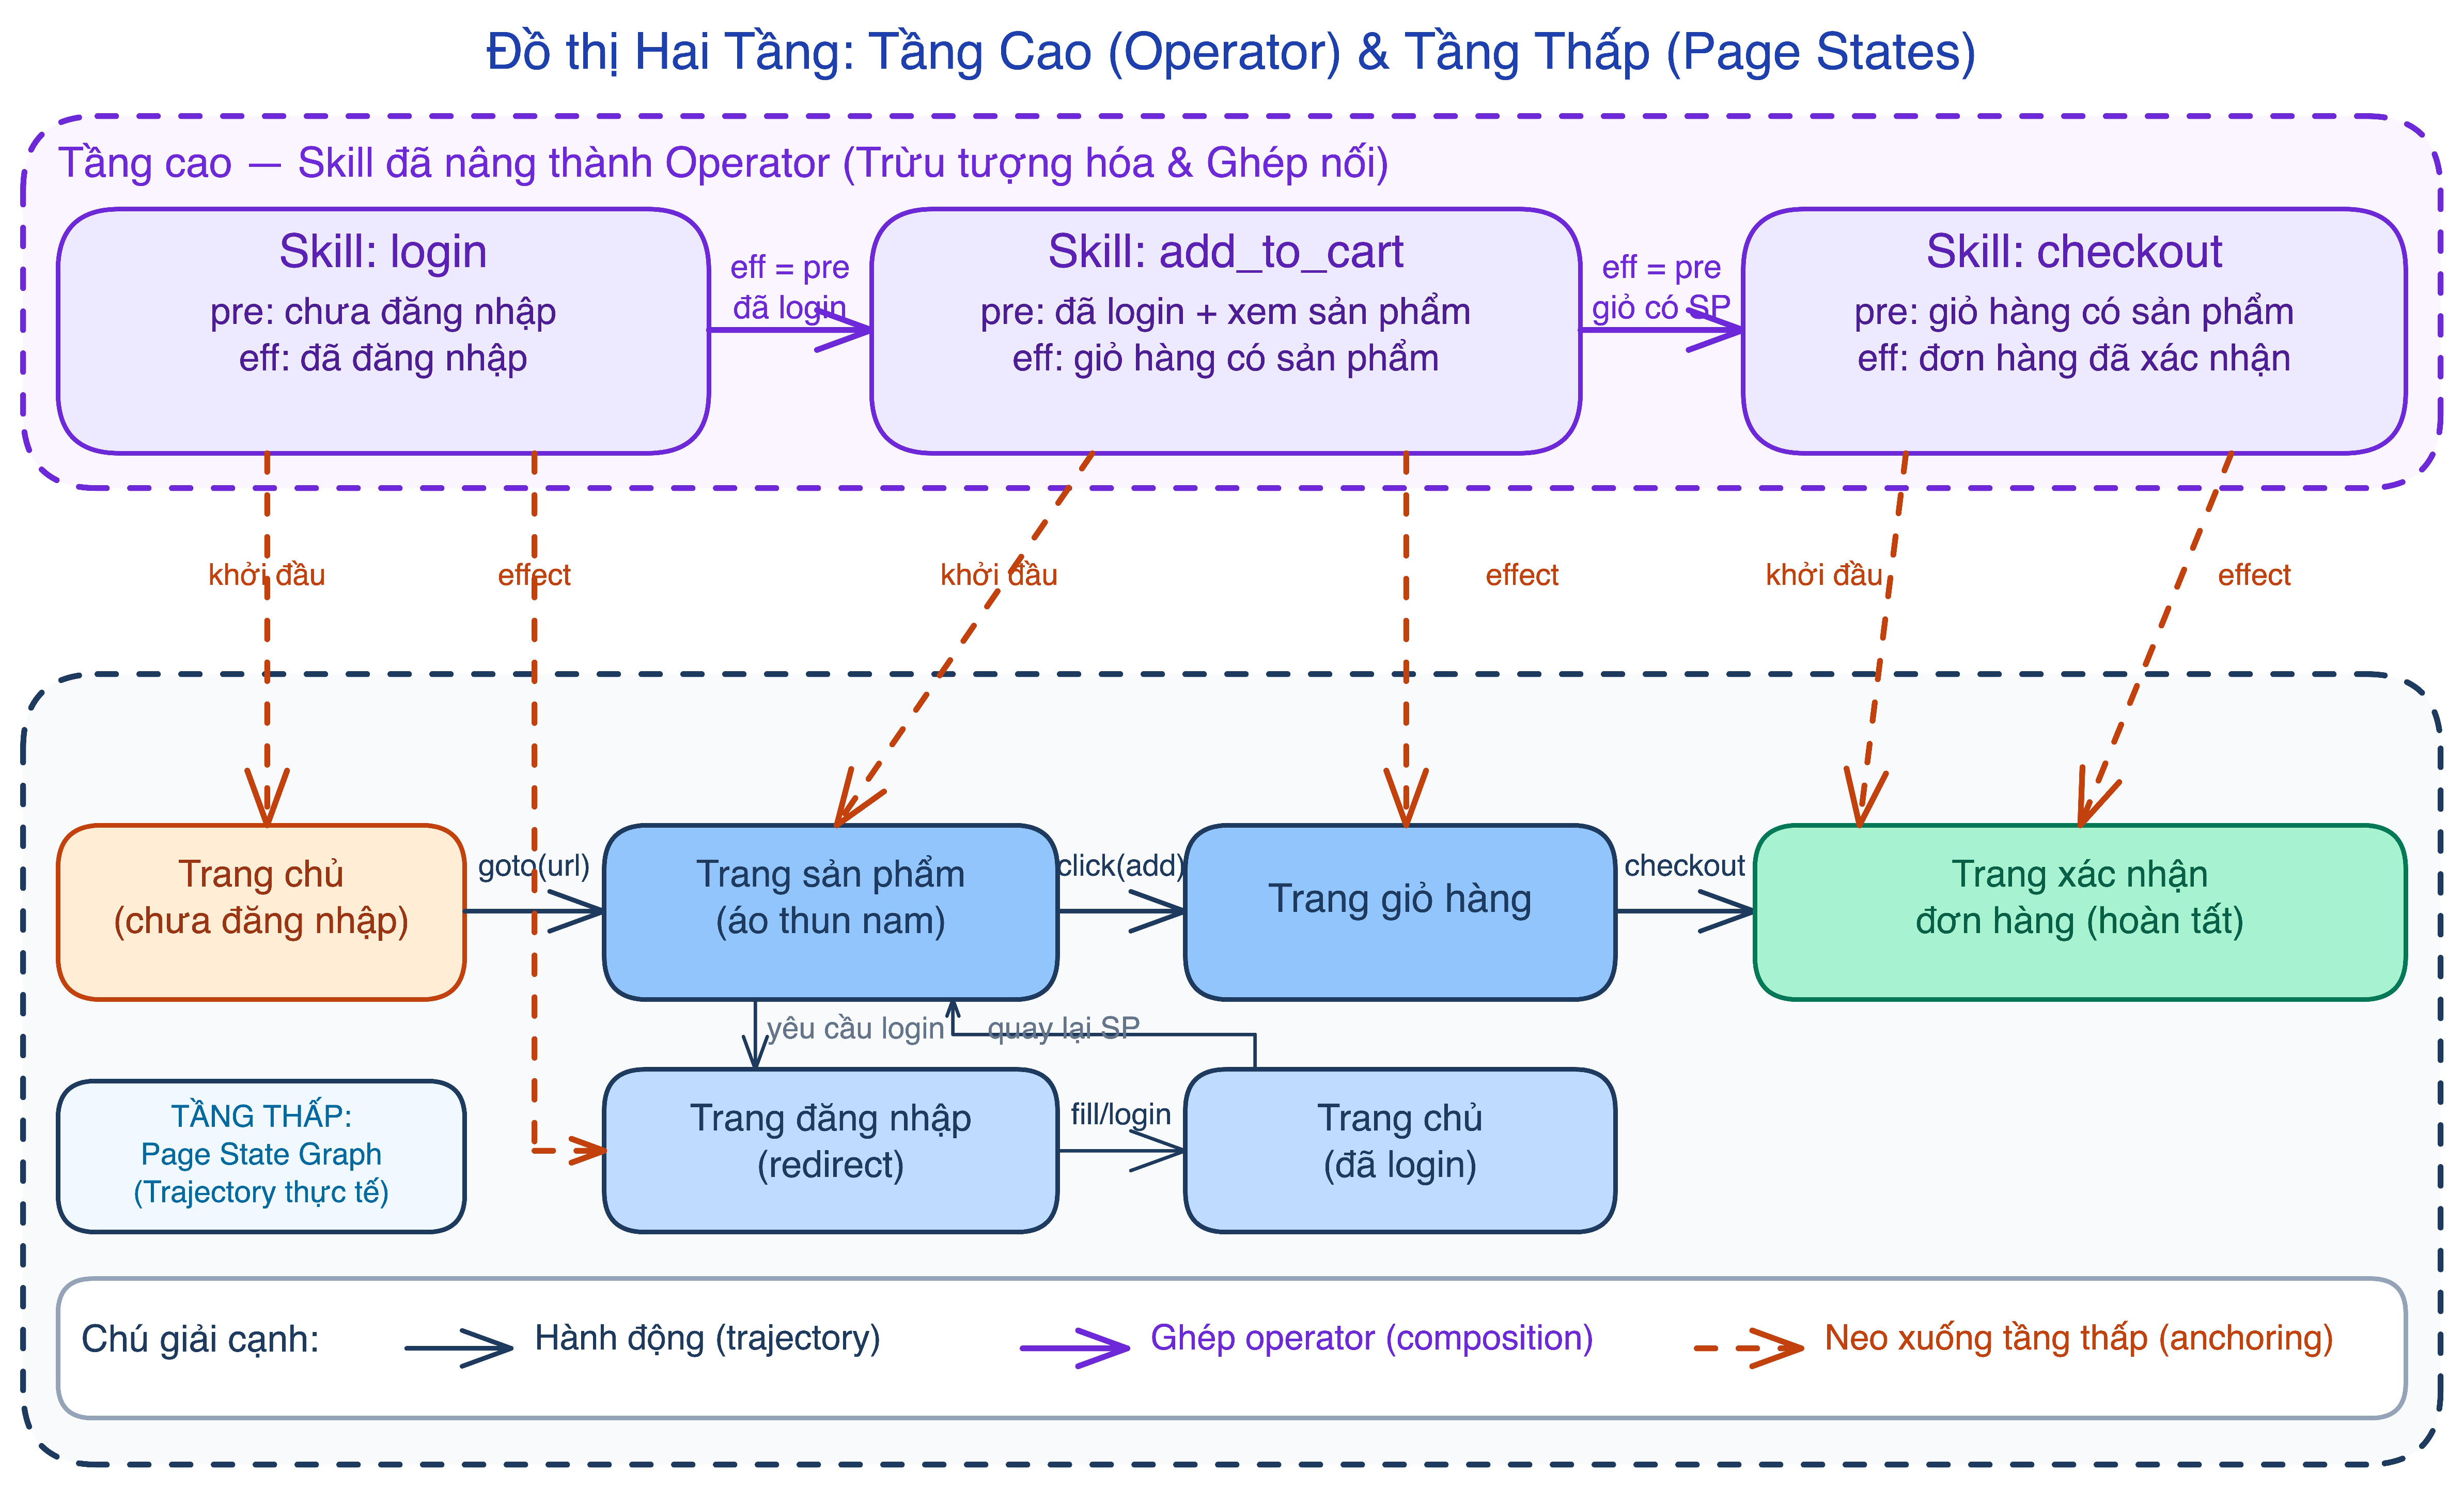
\includegraphics[width=0.95\textwidth]{Figures/fig_twolevel.pdf}
\caption[Đồ thị hai tầng]{Đồ thị hai tầng. Tầng thấp ghi nhận các trạng thái trang (page state) đã thăm và các cạnh quỹ đạo tương tác (hành động) giữa chúng; tầng cao biểu diễn các skill được nâng cấp thành các operator lập kế hoạch và nối với nhau bằng các cạnh ghép (nơi effect của operator trước khớp với precondition của operator sau). Các skill được neo vào tầng thấp thông qua các liên kết trừu tượng hóa và initiation/effect.}
\label{fig:twolevel}
\end{figure}

\subsection{Mô hình hóa website như một quá trình quyết định}

Chúng tôi mô hình hóa website như một Quá trình Quyết định Markov quan sát được một phần (POMDP)~\cite{kaelbling1998pomdp}: agent không bao giờ nhìn thấy toàn bộ trạng thái của máy chủ, mà chỉ thấy phần giao diện đang được hiển thị. Tại mỗi bước, agent nhận được một quan sát $o = (u, x)$, trong đó $u$ là URL hiện tại và $x$ là \emph{cây trợ năng} (accessibility tree - axtree) của trang. Axtree đóng vai trò như một bản tuần tự hóa dưới dạng văn bản (text serialization) của các phần tử giao diện đang hiển thị, trong đó mỗi phần tử được gắn một mã định danh ổn định.

Cách biểu diễn quan sát bằng axtree và việc quy các thao tác giao diện về một tập lệnh hữu hạn không phải là đóng góp của khóa luận: đây là quy ước chuẩn của WebArena~\cite{zhou2024webarena} và bộ công cụ BrowserGym~\cite{dechezelles2025browsergym} mà HSGE kế thừa. Trên nền đó, agent tương tác với môi trường thông qua một không gian hành động cố định $\mathcal{A}$ (Bảng~\ref{tab:actions}). Không gian này gồm các thao tác với phần tử, điều hướng, quản lý tab và hai hành động kết thúc phiên: trả lời người dùng hoặc tuyên bố tác vụ bất khả thi. Một \emph{quỹ đạo tương tác} (trajectory) là chuỗi $\tau = \langle (o_0, a_0), (o_1, a_1), \dots \rangle$ được sinh ra trong quá trình thực thi một tác vụ.

\begin{table}[H]
\centering
\caption[Action space của solver]{Không gian hành động của solver. Các đối số phần tử tham chiếu mã định danh hiển thị trong accessibility tree. Nhóm ba hành động không tác động lên trạng thái trang được tách riêng vì chúng chỉ tồn tại để gỡ bế tắc thao tác, và về sau chính sự phân biệt này quyết định một cổng lọc dữ liệu (Mục~\ref{sec:method-data}).}
\label{tab:actions}
\small
\begin{tabular}{@{}L{5.4cm} L{7.8cm}@{}}
\toprule
\textbf{Hành động} & \textbf{Ý nghĩa} \\
\midrule
\texttt{click(id)} & Nhấn vào phần tử \texttt{id}. \\
\texttt{fill(id, text)} & Nhập chuỗi \texttt{text} vào ô \texttt{id}. \\
\texttt{select\_option(id, opt)} & Chọn tùy chọn \texttt{opt} trong danh sách thả xuống \texttt{id}. \\
\texttt{press(id, key)} & Gửi phím tắt đến phần tử \texttt{id}. \\
\texttt{goto(path)}, \texttt{go\_back()} & Điều hướng tới một đường dẫn \emph{tương đối} trên chính website hiện tại / Quay lại trang trước. \\
\texttt{new\_tab()}, \texttt{tab\_focus(i)}, \texttt{tab\_close()} & Quản lý tab trình duyệt. \\
\addlinespace
\texttt{scroll(dx, dy)} & Cuộn trang; dùng để đưa một phần tử ngoài khung nhìn vào trạng thái thao tác được. \\
\texttt{hover(id)} & Di chuột lên phần tử \texttt{id}. \\
\texttt{noop(ms)} & Chờ trang ổn định. \\
\addlinespace
\texttt{send\_msg\_to\_user(text)} & Kết thúc: Phản hồi câu trả lời hoặc báo cáo hoàn thành. \\
\texttt{report\_infeasible(reason)} & Kết thúc: Khẳng định tác vụ không thể thực hiện. \\
\bottomrule
\end{tabular}
\end{table}

Ba hành động \texttt{scroll}, \texttt{hover} và \texttt{noop} vốn được lớp
thực thi hỗ trợ ngay từ đầu nhưng ban đầu không được mô tả trong prompt, nên
mô hình không bao giờ dùng tới. Hệ quả là khi một thao tác thất bại vì phần tử
chưa ở trạng thái sẵn sàng, phương án duy nhất mà mô hình còn lại là nhấn
lại chính phần tử đó. Việc bổ sung chúng vào tài liệu hành động, kèm chỉ dẫn
tường minh rằng một lỗi quá hạn chờ nghĩa là phần tử có tồn tại nhưng chưa
thao tác được, là một sửa chữa xuất phát từ số liệu của lần chạy thật
(Mục~\ref{sec:exp-analysis}).

Một chi tiết khác của không gian hành động là \texttt{goto} luôn nhận đường
dẫn tương đối. Địa chỉ máy chủ của một bản triển khai WebArena chỉ là ngẫu
nhiên của nơi nó được dựng lên, trong khi dữ liệu của khóa luận được thu thập
trên một máy chủ và được đánh giá trên một máy chủ hoàn toàn khác. Vì vậy, mọi
URL xuất hiện trong prompt cũng như mọi đích đến của \texttt{goto} đều được
lược bỏ phần gốc (origin) trước khi hiển thị hoặc trước khi trở thành đích
huấn luyện, và phần gốc của trang hiện tại chỉ được ghép trở lại ngay trước
thời điểm hành động được thực thi. Phép biến đổi hai chiều này được áp dụng
thống nhất ở cả ba nơi (solver lúc chạy thật, bộ dựng dataset và bộ viết lại
suy nghĩ), nhờ đó một hành động \texttt{goto} học được trên một bản triển khai
vẫn chạy đúng trên một bản triển khai khác.

\subsection{Tầng thấp: Trạng thái trang và cạnh quỹ đạo}

Tầng thấp của đồ thị lưu giữ các bước tương tác cụ thể: các node đại diện cho những trạng thái trang đã thăm (được định danh bởi URL và giá trị băm (hash) của axtree ban đầu); các cạnh thể hiện những hành động mà agent đã thực sự thực thi giữa các trạng thái đó. Việc băm (hashing) nội dung trang thay vì chỉ dựa vào URL là một cơ chế thiết yếu trong thực tế: hai URL khác nhau thường trỏ đến cùng một nội dung giao diện; nếu chỉ dùng URL, việc thăm lại chúng sẽ làm lãng phí ngân sách khám phá vào những nội dung mà agent đã biết.

\subsection{Tầng cao: Biểu diễn skill như các option}

Một \emph{skill} được định nghĩa là một hành vi có khả năng tái sử dụng và được tham số hóa. Khái niệm này được hình thức hóa dựa trên khung options~\cite{sutton1999options} thành bộ ba $\sigma = \langle I, \pi, \beta \rangle$: tập khởi đầu $I$ (các trạng thái trang mà skill có thể được kích hoạt), chính sách $\pi$ (thủ tục hành động) và điều kiện kết thúc $\beta$. Cụ thể, HSGE biểu diễn mỗi skill thông qua một \emph{thẻ kỹ năng} (skill card). Thẻ này gồm tên, mô tả bằng ngôn ngữ tự nhiên, danh sách các tham số được định kiểu (ví dụ: chuỗi tìm kiếm hoặc giá trị điền form), cùng các liên kết trỏ về những đoạn quỹ đạo thành phần mà từ đó skill được trừu tượng hóa. Các node skill kết nối với trạng thái ở tầng thấp thông qua cạnh khởi đầu và cạnh hiệu ứng, đồng thời nối kết với nhau thông qua cạnh ghép chuỗi để hình thành nên đồ thị tầng cao.

\subsection{Toán tử lập kế hoạch: Precondition và Effect}

Việc lập kế hoạch trực tiếp trên các skill thô là không khả thi do điều kiện áp dụng của chúng chỉ tồn tại ở dạng ngầm định. Do đó, HSGE nâng cấp mỗi skill đã qua kiểm chứng thành một toán tử (\emph{operator}) theo mô hình STRIPS cổ điển~\cite{fikes1971strips}: $\omega = \langle \mathit{pre}, \mathit{eff} \rangle$. Ở đây $\mathit{pre}$ và $\mathit{eff}$ là các tập mệnh đề bằng ngôn ngữ tự nhiên, chẳng hạn ``người dùng đang xem danh sách issue của một dự án''.

Điểm khác biệt so với các bộ lập kế hoạch truyền thống là từ vựng của các mệnh đề không được cố định từ trước. Thay vào đó, các mệnh đề này do LLM tự sinh trong quá trình quy nạp (induction), sau đó được \emph{chuẩn hóa} thành các mã định danh ổn định thông qua một bộ gom cụm dựa trên vector nhúng (embedding) (Mục~\ref{sec:method-semantic}). Cơ chế này đảm bảo rằng các cách diễn đạt khác nhau của cùng một điều kiện sẽ được quy về một mệnh đề duy nhất. Trên nền đó, một \emph{đồ thị toán tử} (operator graph) sẽ hình thành một cạnh nối từ $\omega_1$ sang $\omega_2$ khi một hiệu ứng (effect) của $\omega_1$ thỏa mãn điều kiện tiên quyết (precondition) của $\omega_2$. Các đường đi trên đồ thị này chính là các kế hoạch đa kỹ năng (multi-skill) có thể thực thi được.

\subsection{Phân loại thuật ngữ tác vụ}

Xuyên suốt khóa luận, chúng tôi định nghĩa hai phân cấp tác vụ riêng biệt. \emph{Tác vụ mức thấp} (low-level task) là những chỉ dẫn ngắn, gắn liền với một trang web cụ thể do mô-đun explorer đề xuất trong quá trình thăm trang (ví dụ: ``mở merge request được cập nhật gần nhất''). Ngược lại, \emph{tác vụ ngữ nghĩa} (semantic task) là những mục tiêu dài hạn được kiến tạo từ đồ thị toán tử bằng cách ghép chuỗi ít nhất hai operator. Loại tác vụ này phụ thuộc hoàn toàn vào cấu trúc của đồ thị và chính là sản phẩm cốt lõi của phương pháp đề xuất.

\section{Khám phá có định hướng theo đồ thị}
\label{sec:method-exploration}

Quá trình khám phá tại mỗi bước cần giải quyết ba câu hỏi cốt lõi: di chuyển đến \emph{đâu} tiếp theo, thử nghiệm \emph{điều gì} tại đó, và thực thi \emph{như thế nào}. Hệ thống HSGE phân bổ ba nhiệm vụ này lần lượt cho các thành phần: biên khám phá (frontier), mô-đun đề xuất (explorer) và tác nhân giải quyết (solver).

\subsection{Quản lý frontier}
\label{sec:method-frontier}

\begin{figure}[htbp]
\centering
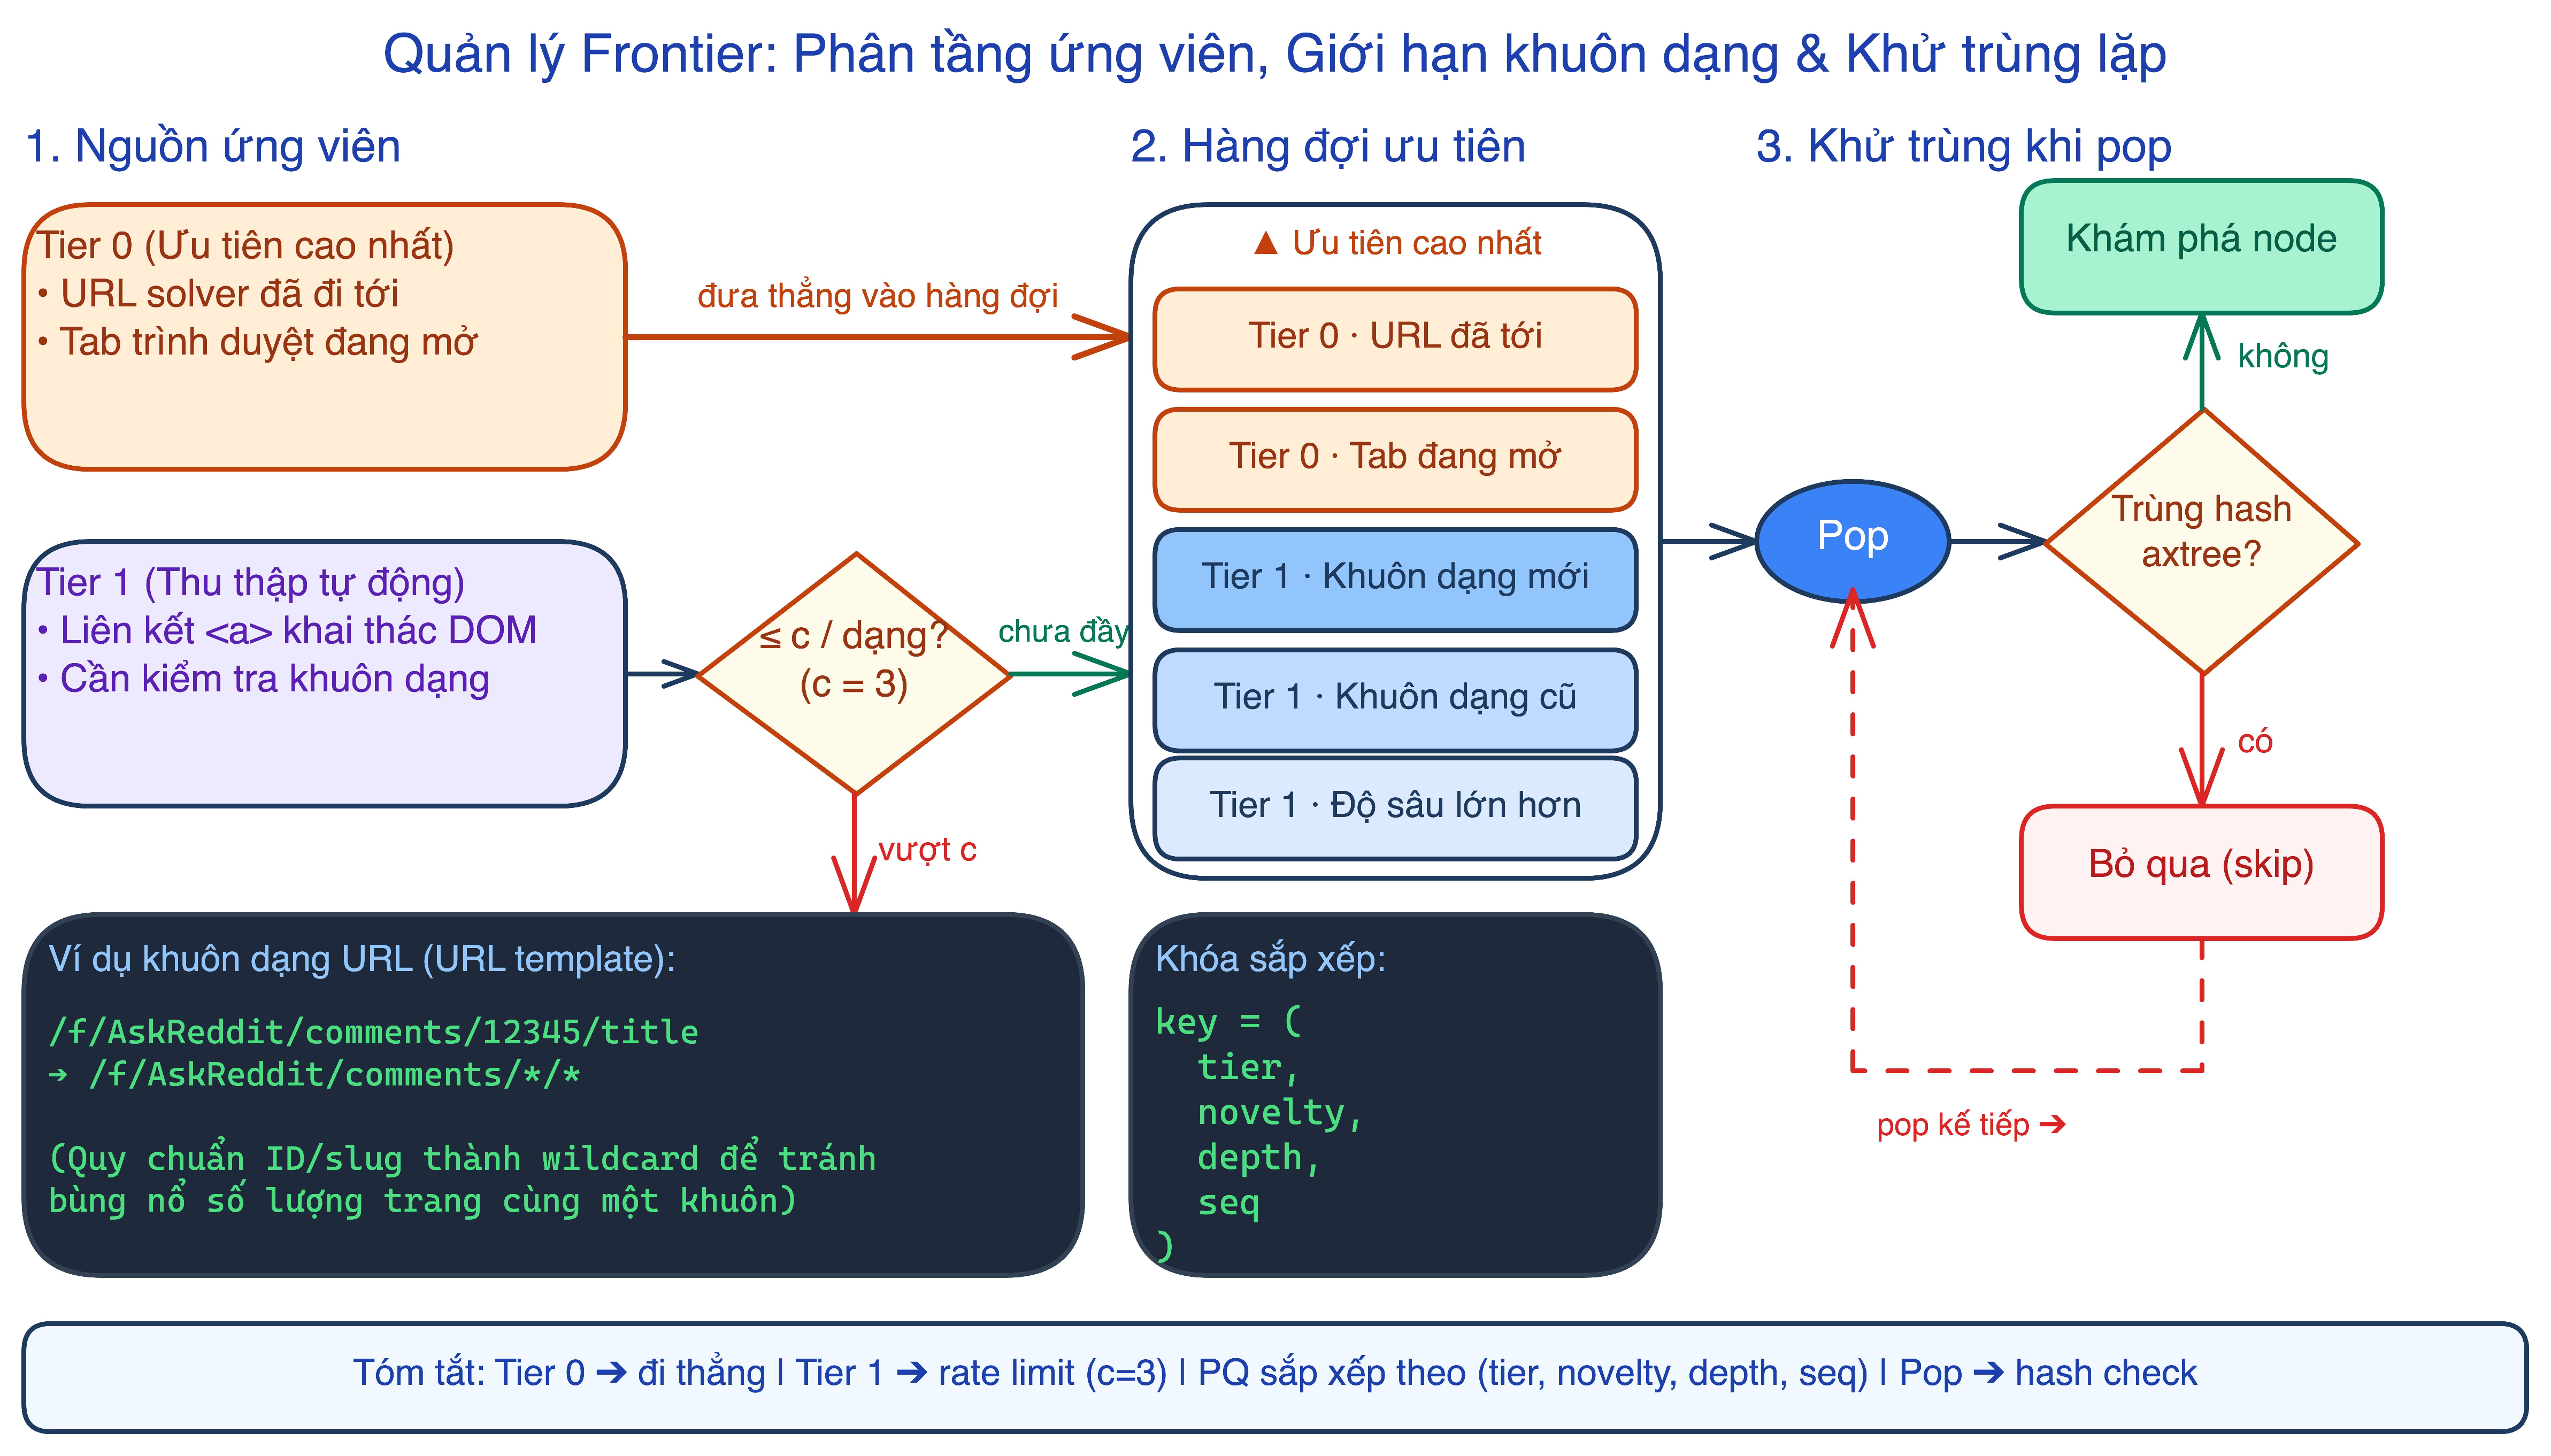
\includegraphics[width=\textwidth]{Figures/fig_frontier.pdf}
\caption[Quản lý frontier]{Quản lý frontier. Hai tầng ứng viên được xử lý theo các cơ chế khác nhau: URL mà solver thực tế đã truy cập được đưa trực tiếp vào hàng đợi, trong khi các siêu liên kết (hyperlink) khai thác từ trang phải vượt qua rào lọc theo khuôn dạng (template). Hàng đợi sắp xếp các ứng viên ưu tiên theo tầng, tiếp đến là độ mới của định dạng URL, và cuối cùng là độ sâu. Một node khi được lấy ra vẫn sẽ bị bỏ qua nếu nội dung trang có giá trị băm (hash) trùng lặp với một trang đã thăm trước đó.}
\label{fig:frontier}
\end{figure}

Frontier được cấu trúc như một hàng đợi ưu tiên dành cho các URL ứng viên, phân làm hai tầng (Hình~\ref{fig:frontier}). \emph{Tầng 0} bao gồm các URL mà agent thực tế đã truy cập khi giải quyết tác vụ, cùng với các trang đang mở trên tab; việc agent truy cập thành công bản thân nó đã là minh chứng cho mức độ liên quan của trang, nên nhóm này luôn được lấy ra trước. \emph{Tầng 1} lưu trữ các siêu liên kết được trích xuất từ cấu trúc DOM của mỗi trang đã thăm. Việc khai thác hyperlink là bắt buộc; nếu không, sự mở rộng của biên khám phá sẽ phụ thuộc hoàn toàn vào các thao tác điều hướng sinh ra khi giải quyết tác vụ. Điều này dẫn đến một rủi ro hệ thống (sẽ được phân tích kỹ hơn ở Chương~\ref{ch:discussion}): nếu một trang web chỉ bao gồm các tác vụ tra cứu thông tin, nó sẽ không cung cấp thêm bất kỳ URL mới nào cho biên khám phá.

Tuy nhiên, số lượng liên kết được trích xuất thường rất ồ ạt và dễ bị áp đảo bởi các trang có cấu trúc tương đồng (ví dụ: mọi bài đăng, bình luận, trang cá nhân trên một diễn đàn thường dùng chung một khuôn mẫu trang). Để ngăn chặn tình trạng quá tải hàng đợi, mỗi URL sẽ được chuẩn hóa thành một \emph{khuôn dạng URL} (URL template): loại bỏ giao thức (scheme), chuỗi truy vấn (query) và phân mảnh (fragment); các đoạn đường dẫn đóng vai trò định danh cùng mọi thành phần phía sau sẽ được thay thế bằng ký tự đại diện. Ví dụ:
\begin{center}
\texttt{/f/AskReddit/comments/12345/title}
$\;\rightarrow\;$
\texttt{/f/AskReddit/comments/*/*}.
\end{center}
Mỗi template chỉ được phép truy cập tối đa $c$ trang; các lượt chạy trong khóa luận dùng $c = 3$ cho tầng 1, và toàn bộ tham số chạy cùng giá trị đã dùng được liệt kê ở Phụ lục~\ref{app:design-params}. Giới hạn này được kiểm tra theo cơ chế đánh giá lười (lazy evaluation) ngay tại thời điểm lấy URL ra khỏi hàng đợi, bởi tần suất xuất hiện của một template sẽ tăng dần theo thời gian chạy (run). Tại tầng 1, các ứng viên thuộc template chưa từng gặp sẽ được ưu tiên trước, tiếp đến là các trang ở mức nông hơn, và cuối cùng là thứ tự chèn.

Điểm cần nói rõ là tầng 0 cũng chịu một trần theo template, chỉ với giá trị
rộng hơn ($c = 8$), chứ \emph{không} được miễn trừ. Việc miễn trừ hoàn toàn cho
tầng 0 là thiết kế ban đầu và nó đã hỏng theo một cách khá đặc trưng: khi
solver giải một tác vụ bên trong một chuỗi bình luận, mọi URL nó chạm tới trong
lúc giải đều được đẩy lên đầu hàng đợi mà không qua bộ lọc nào, khiến một
diễn đàn duy nhất chiếm 58 trên 158 node của một lượt chạy thật. Nói cách khác,
bằng chứng ``agent đã đi tới đó'' đủ để \emph{ưu tiên} một trang, nhưng không
đủ để cho nó quyền chiếm ngân sách khám phá không giới hạn.

Thuật toán~\ref{alg:frontier} tóm tắt vòng lặp này. Việc chống trùng lặp được
thực hiện ở ba mức khác nhau, vì cùng một trang có thể xuất hiện dưới ba dạng
khác nhau. Thứ nhất, mỗi URL được chuẩn hóa (bỏ phân mảnh, hạ chữ thường phần
giao thức và tên máy, bỏ dấu gạch chéo cuối) trước khi đối chiếu với tập đã
thăm; chuỗi truy vấn được \emph{giữ lại}, bởi hai giá trị truy vấn khác nhau
thường thực sự là hai trang khác nhau. Thứ hai, sau khi trình duyệt điều hướng
xong, URL thực tế mà nó dừng lại cũng được đối chiếu, để bắt các trường hợp
chuyển hướng về một trang đã thăm. Thứ ba, mã băm nội dung của cây trợ năng
ban đầu được đối chiếu, để bắt những URL khác nhau nhưng hiển thị nội dung
giống hệt. Node nào trùng theo một trong ba mức đều bị bỏ qua, vì thăm lại nó
tiêu tốn trọn một lô lời gọi LLM mà không mang lại phát hiện nào.

\begin{algorithm}[H]
\caption{Vòng khám phá có định hướng theo đồ thị}
\label{alg:frontier}
\begin{algorithmic}[1]
\State $F \gets$ hàng đợi ưu tiên khởi tạo với URL hạt giống $r$; $V \gets \emptyset$
\While{$F \neq \emptyset$ \textbf{và} chưa vượt quá ngân sách node}
  \State $u \gets \textsc{Pop}(F)$ \Comment{khóa: (tầng, độ mới template, độ sâu, thứ tự)}
  \If{template của $u$ đã đạt trần của tầng đó} \textbf{continue} \EndIf
  \State $o \gets \textsc{Load}(u)$ \Comment{lỗi tải trang: ghi log, bỏ qua node, không dừng run}
  \If{$\textsc{Landed}(o) \in V$ \textbf{hoặc} $\textsc{Hash}(o) \in V$} \textbf{continue} \EndIf
  \State $V \gets V \cup \{\textsc{Landed}(o), \textsc{Hash}(o)\}$
  \State $D \gets \emptyset$ \Comment{các task đã giải được tại node này}
  \For{task $t \in \textsc{Explorer}(o)$} \Comment{low-level task, Mục~\ref{sec:method-lowlevel}}
    \State $\tau \gets \textsc{Solver}(u, t)$; ghi episode nhãn \texttt{LOCAL}
    \If{$\tau$ thành công} $\textsc{Discovery}(\tau)$; $D \gets D \cup \{t\}$ \EndIf
    \State thêm các URL đạt tới trong $\tau$ vào $F$ ở tầng 0
  \EndFor
  \For{task $t \in D$} \Comment{lấy mẫu không tiền tố, Mục~\ref{sec:method-unprefixed}}
    \State $\tau \gets \textsc{Solver}(r, t)$; ghi episode nhãn \texttt{UNPREFIXED}
    \If{$\tau$ thành công} $\textsc{Discovery}(\tau)$ \EndIf
  \EndFor
  \For{task $t \in \textsc{SemanticTasks}(u)$} \Comment{chuỗi operator + seed, Mục~\ref{sec:method-semantic}}
    \State $\tau \gets \textsc{Solver}(u, t)$; ghi episode nhãn \texttt{GOAL}
  \EndFor
  \State khai thác hyperlink của $u$; thêm vào tầng 1 theo trần template
  \State ghi sản phẩm trung gian và điểm kiểm tra (checkpoint) của node
\EndWhile
\end{algorithmic}
\end{algorithm}

\subsection{Đề xuất tác vụ mức thấp (low-level task)}
\label{sec:method-lowlevel}

Tại mỗi trang thuộc biên khám phá, một mô-đun \emph{explorer} vận hành lõi LLM sẽ đề xuất tối đa $k$ tác vụ cụ thể gắn liền với nội dung trang; giá trị mặc định là $k = 6$, còn các lượt chạy thu thập dữ liệu của khóa luận dùng $k = 9$ (Phụ lục~\ref{app:design-params}). Các đề xuất này được biểu diễn dưới dạng dữ liệu có cấu trúc, đi kèm trường phân loại tường minh nhận một trong bốn giá trị: \texttt{INFO} (tra cứu một thông tin), \texttt{NAV} (đi tới một trang cụ thể), \texttt{MOD} (thay đổi nội dung hoặc trạng thái) và \texttt{COMPOSITE} (một mục tiêu tự thân đòi hỏi nhiều thao tác mới thỏa mãn, chẳng hạn ``mua con chuột không dây rẻ nhất còn hàng''). Cách làm này thay cho việc yêu cầu LLM trả về văn bản tự do (free-text) kèm thẻ gắn phân loại -- một quy ước mà thử nghiệm trên website thật cho thấy mô hình không tuân thủ ổn định (Mục~\ref{sec:disc-guardrails}).

Nhóm \texttt{COMPOSITE} có vai trò riêng và được prompt yêu cầu đặt lên đầu danh sách: đây là nhóm duy nhất trong bốn nhóm mà một tác vụ đơn lẻ đã trải qua nhiều trạng thái trang, nên nó là nguồn sinh ra các kỹ năng có thể tái sử dụng và ghép chuỗi. Một quy tắc cụ thể đi kèm là khi trang hiện tại có biểu mẫu nhiều trường, explorer không được đề xuất tác vụ chỉ điền một trường đơn lẻ, mà phải đề xuất một tác vụ hoàn tất trọn vẹn biểu mẫu đó theo đúng mục đích của nó. Ngoài ra, mọi tác vụ liên quan tới tài khoản và xác thực (đăng nhập, đăng xuất, đăng ký, đổi mật khẩu, xóa tài khoản) đều bị cấm tuyệt đối ở mọi chế độ, bởi phiên làm việc vốn đã được xác thực sẵn và tài khoản được dùng chung giữa các lượt chạy.

Việc phân loại đóng vai trò then chốt đối với chế độ \emph{chỉ đọc} (read-only) dành cho các website dùng chung. Ở chế độ này, các tác vụ \texttt{MOD} cũng như mọi tác vụ mô hình không phân loại được đều bị loại bỏ theo nguyên tắc an toàn đóng mặc định (fail-closed), nhằm phòng ngừa những tác vụ thay đổi trạng thái bị ngụy trang.

Hệ thống áp dụng ba cơ chế để kiểm soát thành phần và tính đa dạng của danh sách đề xuất. Thứ nhất, explorer duy trì trạng thái xuyên suốt toàn bộ quá trình chạy và ghi nhớ mọi tác vụ đã từng đề xuất; các đề xuất gần nhất sẽ được đưa ngược lại vào prompt dưới dạng ngữ cảnh phủ định (negative context), đồng thời các phiên bản gần trùng lặp sẽ bị loại bỏ ở cấp độ mã nguồn. Thiếu đi cơ chế này, một tỷ lệ lớn các đề xuất sẽ thoái hóa thành những lệnh điều hướng menu lặp lại trên mọi trang (Mục~\ref{sec:disc-exploration}).

Thứ hai, hai nhóm tác vụ bị giới hạn số lượng \emph{không điều kiện}, bất kể ngân sách $k$ còn trống hay không: tối đa một tác vụ \texttt{NAV} và tối đa hai tác vụ \texttt{INFO} cho mỗi trang. Lý do của trần \texttt{NAV} là các tác vụ \texttt{COMPOSITE} và \texttt{MOD} vốn đã tự điều hướng sang trang mới trong lúc thao tác, nên một tác vụ điều hướng thuần túy chỉ cần giữ lại như một khoản dự phòng. Lý do của trần \texttt{INFO} đến từ số liệu của một lượt chạy thật: khi nhóm này chỉ bị cắt lúc danh sách vượt ngân sách, các trang đề xuất ít tác vụ sẽ để lọt toàn bộ \texttt{INFO}, và kết quả là \texttt{INFO} chiếm 49\% tổng số phiên thành công, trong đó phần lớn kết thúc bằng một câu trả lời mà không có bất kỳ thao tác trình duyệt nào. Đó là dữ liệu dạy mô hình \emph{trả lời}, không phải dạy mô hình \emph{hành động}, nên nó cần được giữ ở mức vừa đủ chứ không phải càng nhiều càng tốt.

Thứ ba, khi danh sách vẫn vượt quá $k$ sau hai bước trên, thứ tự giữ lại được quy định tường minh: trước hết là một lượng \texttt{COMPOSITE} dự trữ, rồi tới toàn bộ \texttt{MOD}, rồi một lượng \texttt{INFO} dự trữ, rồi \texttt{NAV}, và sau cùng mới tới phần \texttt{COMPOSITE} dôi ra, các tác vụ không phân loại được và phần \texttt{INFO} dôi ra. Trật tự này bảo đảm cả hai điều: nhóm sinh ra skill không bao giờ bị cắt hết, còn nhóm chỉ đọc luôn giữ được một phần đại diện trong dữ liệu.

Khi seed năng lực của website đã được suy ra (Mục~\ref{sec:method-seed}), mô tả website cùng danh sách năng lực còn được đưa vào prompt của explorer như ngữ cảnh bổ sung, kèm chỉ dẫn rằng chúng không được thay thế các tác vụ gắn với trang hiện tại. Mục đích là để các tác vụ mức thấp bám sát mục đích thật của website, thay vì chỉ mô tả những gì trang đang hiển thị.

Các tác vụ đề xuất này được \emph{chủ đích} giữ ở mức thấp: mỗi tác vụ nằm trọn vẹn trong phạm vi chức năng của một trang đơn lẻ. Vai trò cốt lõi của chúng là tạo ra các quỹ đạo tương tác đa dạng, đóng vai trò là nguồn dữ liệu thô để từ đó hệ thống trích xuất các kỹ năng, và sau cùng là nền tảng để tổng hợp thành các tác vụ ngữ nghĩa.

\subsection{Tác nhân giải quyết (Solver)}
\label{sec:method-solver}

\begin{figure}[htbp]
\centering
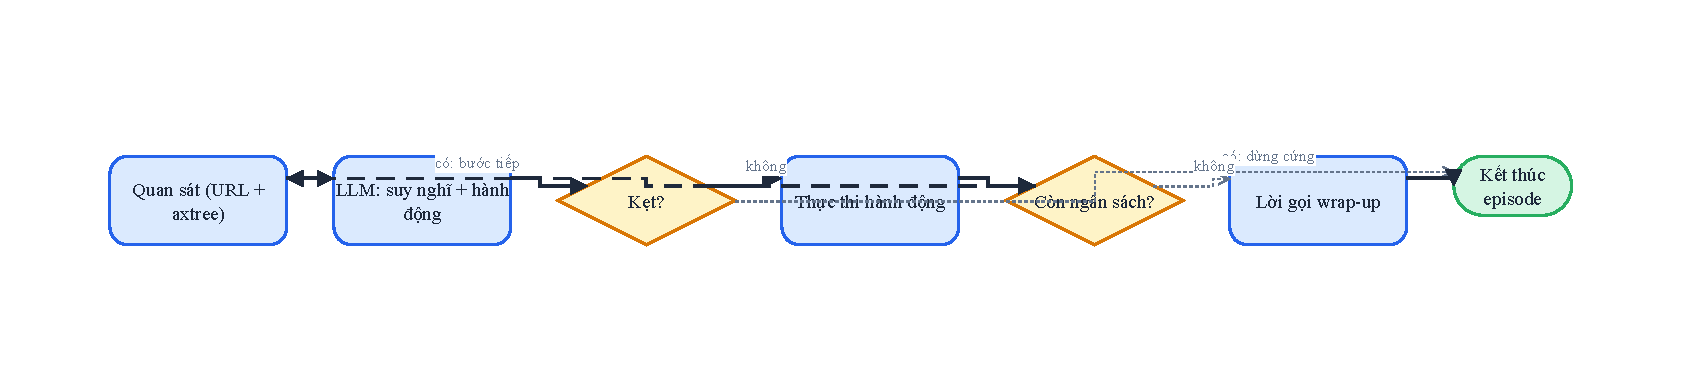
\includegraphics[width=\textwidth]{Figures/fig_solver.pdf}
\caption[Vòng lặp Solver với chốt chặn cấu trúc]{Vòng lặp quan sát, suy nghĩ, hành động của solver. Cơ chế chốt chặn vòng lặp kẹt (stuck-loop) sẽ chấm dứt ngay episode khi các hành động liên tục lặp lại trên cùng một đối tượng đích mà không tạo ra bất kỳ sự thay đổi quan sát nào; khi cạn kiệt ngân sách bước nhảy, hệ thống gọi một hàm tổng kết (wrap-up) duy nhất, chỉ cho phép tuyên bố hoàn thành hoặc báo cáo bất khả thi.}
\label{fig:solver}
\end{figure}

\emph{Solver} hoạt động dựa trên vòng lặp agent theo kiến trúc ReAct~\cite{yao2023react}, được phác họa ở Hình~\ref{fig:solver}. Tại mỗi bước, nó tiếp nhận mục tiêu, URL hiện tại (dạng tương đối), cây trợ năng (đã được giới hạn ở 6000 ký tự, kèm dấu hiệu cắt tường minh), một mục báo lỗi của hành động liền trước, và một khung cửa sổ chứa sáu hành động gần nhất. Mỗi hành động trong cửa sổ đó đều đi kèm kết quả quan sát được (``đang ở $\langle$url$\rangle$'', ``trang đã đổi'', ``không đổi'', hoặc ``hành động thất bại: $\langle$lỗi$\rangle$'') nhằm giúp mô hình phân biệt được sự tiến triển so với việc không tạo ra tiến triển. Mục báo lỗi \emph{luôn hiện diện} trong prompt và mang giá trị ``(none)'' khi không có lỗi, thay vì chỉ xuất hiện ở những bước hiếm hoi có lỗi; nhờ vậy nó là một phần cố định của định dạng mà mô hình học cách tra cứu. Tiếp theo, solver đưa ra dòng suy luận và thực thi một hành động thuộc Bảng~\ref{tab:actions}.

Một hành động bị lớp thực thi từ chối vẫn được ghi vào lịch sử như mọi hành động khác, với kết quả là ``thất bại'' và không có tiến triển. Chi tiết này quan trọng hơn vẻ ngoài của nó: trước đây một hành động lỗi được bỏ qua hoàn toàn, khiến cả hai cơ chế chống lặp bên dưới không nhìn thấy gì, và trong một lượt chạy thật đã có 118 phiên tiêu trọn ngân sách để phát đi phát lại một cú nhấp mà phần tử đích không bao giờ ở trạng thái thao tác được.

Vòng lặp của solver được kiểm soát bởi ba cơ chế chốt chặn cấu trúc, mỗi cơ chế bắt một dạng bế tắc khác nhau.

\textbf{Chốt chặn theo đối tượng đích.} Solver theo dõi xem mỗi hành động có làm thay đổi quan sát hay không và tác động lên đối tượng đích nào. Một chuỗi các hành động cuối cùng nhắm vào \emph{cùng một đối tượng đích} mà \emph{không tạo ra sự thay đổi quan sát} trước hết sẽ kích hoạt một cảnh báo chèn thẳng vào prompt (sau hai lần), rồi tới một lệnh chấm dứt lập tức (hard stop) nếu hành vi vẫn tiếp diễn (sau bốn lần). Thiết kế hai mức này xuất phát từ một quan sát trên website thật: cảnh báo bằng văn bản không đủ để mô hình ngừng click vào một phần tử trơ (unresponsive), như trình bày ở Mục~\ref{sec:disc-guardrails}. Việc ràng buộc thêm yếu tố ``không có sự thay đổi quan sát'', thay vì chỉ so khớp chuỗi hành động, giúp cơ chế chốt chặn không bị kích hoạt sai (false positive). Nhờ đó nó không cắt nhầm những chuỗi thao tác hợp lệ cần tái sử dụng một phần tử xuyên suốt nhiều trang khác nhau.

\textbf{Chốt chặn theo độ mới của quan sát.} Cơ chế trên chỉ nhận ra bế tắc khi mô hình lặp lại \emph{cùng} một đối tượng đích. Trong thực tế còn một dạng bế tắc khác, khi mô hình liên tục đổi đối tượng nhưng không bao giờ chạm tới một trang mới, tức nó đang loanh quanh chứ không đang tiến. Vì vậy solver ghi lại tập các quan sát đã đạt tới và đếm số bước liên tiếp không đưa lại quan sát nào mới; vượt qua ngưỡng cảnh báo (bốn bước) thì prompt được chèn một lời nhắc đổi hướng tiếp cận, vượt qua ngưỡng dừng (tám bước) thì episode kết thúc.

\textbf{Lời gọi tổng kết.} Khi vòng lặp kết thúc mà chưa có hành động kết thúc nào được chọn, dù vì cạn ngân sách bước hay vì một trong hai chốt chặn trên, solver thực thi một lời gọi \emph{tổng kết} (wrap-up call) cuối cùng. Lời gọi này thuần túy ở định dạng văn bản và chỉ được phép phản hồi \texttt{send\_msg\_to\_user} (tuyên bố hoàn thành) hoặc \texttt{report\_infeasible} (báo cáo bất khả thi); mọi phản hồi khác đều bị loại bỏ. Một chi tiết đáng lưu ý là prompt tổng kết nói đúng \emph{lý do thật} khiến episode dừng, bởi hai chốt chặn thường bắn sớm hơn ngân sách rất nhiều; nếu vẫn nói với mô hình rằng nó đã cạn ngân sách thì mô hình sẽ chép lại lời đó, và một lượt chạy thật đã ghi nhận những phiên dừng ở bước thứ năm nhưng báo cáo lý do bất khả thi là ``ngân sách hành động đã cạn''.

Lý do dừng này được lưu lại cùng episode, vì nó phân biệt hai tình huống trông giống hệt nhau trong dữ liệu. Một báo cáo bất khả thi mà tác nhân tự đưa ra \emph{trong lúc} đang giải là một kết luận; cũng câu đó nhưng đến từ lời gọi tổng kết sau khi tác nhân đã bị chặn lại chỉ là một lời biện minh sau sự việc. Trạng thái bất khả thi được xem là một kết quả hợp lệ ở mức cao nhất (first-class outcome): nó không bao giờ được thực thi trên trình duyệt, không bao giờ được thử lại và không tham gia vào quá trình phát hiện skill, nhưng loại thứ nhất được giữ lại làm tín hiệu huấn luyện dạy mô hình biết khi nào nên dừng, còn loại thứ hai bị loại khỏi tập dữ liệu (Mục~\ref{sec:method-data}).

Sau cùng, việc tác nhân tự tuyên bố hoàn thành không đủ để một phiên được ghi là thành công nếu tác vụ thuộc nhóm thay đổi trạng thái. Với một tác vụ \texttt{MOD} hoặc \texttt{COMPOSITE}, hệ thống yêu cầu thêm một điều kiện kiểm tra được bằng mã: phải có ít nhất một hành động đã thực sự làm trang thay đổi. Điều kiện này sinh ra từ một phiên thật, nơi tác vụ ``gửi email xác nhận cho đơn hàng \#000000299'' được tuyên bố hoàn thành ngay ở bước đầu tiên, không một thao tác trình duyệt nào, với lý do rằng email ``đã được gửi rồi''. Các tác vụ \texttt{INFO} và \texttt{NAV} không chịu ràng buộc này, bởi trả lời ngay trên trang đích chính là hình dạng đúng của chúng.

Cuối cùng, khi tác vụ là một mục tiêu ngữ nghĩa nhiều bước, solver có thể được vận hành ở chế độ \emph{bám subgoal}: một thành phần lập kế hoạch phân rã mục tiêu thành từ hai tới năm subgoal có thứ tự, và tại mỗi bước prompt chỉ trưng ra subgoal hiện tại kèm yêu cầu chỉ làm việc trên subgoal đó. Con trỏ subgoal tiến lên khi mô hình phát tín hiệu hoàn thành, hoặc tự động tiến sau một số bước trần, và chỉ subgoal cuối cùng mới được phép kết thúc episode.

\subsection{Lấy mẫu không tiền tố (unprefixed sampling)}
\label{sec:method-unprefixed}

Mọi phiên tương tác mô tả cho tới đây đều có \emph{tiền tố}: trước khi giải một
tác vụ, trình duyệt được đưa về đúng trang mà tác vụ đó gắn với, nên tác nhân
bắt đầu ở nơi cần thao tác. Cách làm này là hệ quả tự nhiên của việc explorer
đề xuất tác vụ theo từng trang, nhưng nó tạo ra một sai lệch nghiêm trọng cho
dữ liệu huấn luyện: phần khó nhất của một tác vụ web thật, tức tìm đường tới
đúng trang, đã bị lược bỏ. Số liệu của một lượt chạy thật cho thấy quy mô của
sai lệch đó: 287 trên 465 quỹ đạo thành công chỉ dài đúng \emph{một} bước, vì
tác nhân đã đứng sẵn ở đích ngay từ đầu.

Vì vậy, sau khi hoàn tất toàn bộ tác vụ mức thấp tại một node, hệ thống thực
hiện thêm một lượt \emph{không tiền tố} theo tinh thần của Go-Browse~\cite{gandhi2026gobrowse}:
mỗi tác vụ \emph{đã giải được} ở node đó được giải lại một lần nữa trên một
trình duyệt mới mở tại trang chủ của website. Quỹ đạo thu về vì thế chứa cả
phần điều hướng lẫn phần thao tác, và được ghi nhận với nhãn \texttt{UNPREFIXED}
ở mức độ khó 2. Vì một tác vụ không tiền tố thực chất là tác vụ cũ cộng thêm
phần tìm đường, nó dùng ngân sách bước của nhóm mục tiêu ngữ nghĩa thay vì
ngân sách của tác vụ cục bộ.

Chỉ những tác vụ đã thành công mới được giải lại. Một tác vụ mà tác nhân không
làm nổi ngay cả khi đứng đúng trang thì cũng không dễ hơn khi phải tự tìm
đường tới đó, nên trả tiền hai lần cho nó chỉ làm hao ngân sách. Đổi lại,
lượt không tiền tố có một tác dụng phụ đáng kể đối với khâu phát hiện kỹ năng:
giải cùng một tác vụ từ hai điểm xuất phát khác nhau cũng chính là cách một
cụm quỹ đạo tích đủ số lần tái xuất hiện để đạt độ chín và trở thành skill.

\section{Phát hiện kỹ năng (Skill Discovery)}
\label{sec:method-skills}

Mọi quỹ đạo tương tác (trajectory) sau khi hoàn tất sẽ đi qua chuỗi xử lý (pipeline) phát hiện gồm bốn giai đoạn: phân cắt quỹ đạo, gom cụm, trừu tượng hóa, và kiểm chứng (Hình~\ref{fig:discovery}).

\begin{figure}[htbp]
\centering
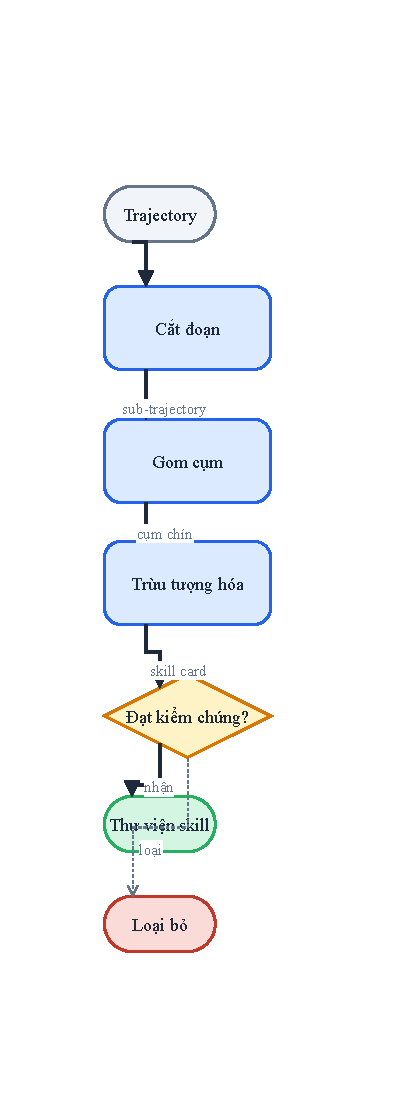
\includegraphics[width=0.48\textwidth]{Figures/fig_discovery.pdf}
\caption[Pipeline phát hiện skill]{Chuỗi xử lý phát hiện kỹ năng. Một trajectory hoàn tất sẽ được phân cắt thành các quỹ đạo con (sub-trajectory), gom cụm, trừu tượng hóa thành thẻ kỹ năng (skill card), và chỉ được lưu vào thư viện nếu vượt qua bước kiểm chứng; nếu không, nó sẽ bị loại bỏ.}
\label{fig:discovery}
\end{figure}

Thuật toán~\ref{alg:discovery} trình bày toàn bộ bốn giai đoạn dưới dạng mã
giả; các mục tiếp theo giải thích chi tiết từng giai đoạn. Điểm cần lưu ý là
pipeline chỉ được kích hoạt trên những quỹ đạo của tác vụ đã giải thành công:
một episode thất bại hoặc kết thúc bằng \texttt{report\_infeasible} không bao
giờ tham gia vào quá trình phát hiện kỹ năng.

\begin{algorithm}[H]
\caption{Phát hiện kỹ năng từ một quỹ đạo tương tác}
\label{alg:discovery}
\begin{algorithmic}[1]
\Require quỹ đạo $\tau$ gồm $n$ bước của một tác vụ đã giải thành công, với
quan sát $o_i = (u_i, x_i)$; thư viện skill $L$; ngưỡng axtree
$\theta_{\mathrm{ax}}$, ngưỡng gom cụm $\theta_{\mathrm{sim}}$, độ chín $m$
\Ensure tập các skill được thu nhận thêm vào $L$
\State $C \gets \emptyset$ \Comment{điểm cắt ứng viên}
\For{$i \gets 1$ \textbf{đến} $n-1$}
  \If{$u_i \neq u_{i-1}$ \textbf{hoặc} $\textsc{Sim}(x_{i-1}, x_i) < \theta_{\mathrm{ax}}$}
    \State $C \gets C \cup \{i\}$
  \EndIf
\EndFor
\State $S \gets \textsc{Arbitrate}(\tau, C)$ \Comment{LLM gộp/xác nhận; điểm cắt không hợp lệ bị bỏ, không phản hồi thì giữ nguyên $C$}
\State $S \gets \textsc{MergeNav}(S)$ \Comment{đoạn một bước thuần điều hướng gộp vào đoạn kề}
\State $A \gets \emptyset$
\For{mỗi quỹ đạo con $\sigma \in S$}
  \State $v \gets \textsc{Embed}(\sigma)$ \Comment{sentence embedding, đã chuẩn hóa $L_2$}
  \State $c \gets \arg\max_j \cos(v, \mu_j)$ \Comment{$\mu_j$ là tâm cụm $j$}
  \If{$L$ chưa có cụm nào \textbf{hoặc} $\cos(v, \mu_c) < \theta_{\mathrm{sim}}$}
    \State $c \gets$ cụm mới, tâm khởi tạo bằng $v$
  \Else
    \State thêm $\sigma$ vào cụm $c$; cập nhật $\mu_c$ theo trung bình lũy tiến rồi chuẩn hóa lại
  \EndIf
  \If{$|\textsc{Members}(c)| \ge m$ \textbf{và} $c$ chưa được trừu tượng hóa}
    \State đánh dấu $c$ đã trừu tượng hóa
    \State $\mathit{card} \gets \textsc{Abstract}(\textsc{Members}(c))$ \Comment{LLM sinh skill card}
    \If{$\textsc{Verify}(\mathit{card})$}
      \State $L \gets L \cup \{\mathit{card}\}$; \; $A \gets A \cup \{\mathit{card}\}$
    \EndIf
  \EndIf
\EndFor
\State \Return $A$
\end{algorithmic}
\end{algorithm}

\subsection{Phân cắt quỹ đạo (Segmentation)}

Một quỹ đạo tương tác thường là sự đan xen của nhiều hành vi khác nhau (như tìm kiếm, lọc, và mở kết quả). Bước phân cắt sẽ chia trajectory ban đầu thành các \emph{quỹ đạo con} (sub-trajectory) có tính liền mạch và đồng nhất về mặt ngữ nghĩa. Các điểm phân cắt tiềm năng (candidate cut points) được xác định dựa trên hai tín hiệu: sự thay đổi của URL và sự sụt giảm độ tương đồng giữa hai cây trợ năng (accessibility tree) liên tiếp. Tín hiệu thứ hai giúp hệ thống nắm bắt được các chuyển đổi trạng thái ngay bên trong một trang (ví dụ: một hộp thoại pop-up xuất hiện) mà không làm thay đổi URL. Sau đó, một LLM sẽ đóng vai trò phân xử các điểm cắt tiềm năng này để đưa ra quyết định gộp hoặc xác nhận phân cắt. Kết quả đầu ra sẽ được kiểm tra tính hợp lệ so với tập ứng viên ban đầu; đồng thời, các đoạn thao tác điều hướng đơn giản (chỉ gồm một bước) sẽ được gộp chung vào quỹ đạo con liền kề.

\subsection{Gom cụm trực tuyến (Streaming Clustering)}

Mỗi quỹ đạo con sẽ được biểu diễn dưới dạng vector nhúng (bằng kỹ thuật sentence embedding~\cite{reimers2019sbert}) và được phân bổ vào một cụm thông qua thuật toán gom cụm phi tham số, hoạt động trực tuyến (streaming) thuộc họ DP-means~\cite{kulis2012dpmeans}. Cụ thể, một đoạn dữ liệu mới sẽ gia nhập cụm gần nhất nếu độ tương đồng cosine (cosine similarity) vượt qua một ngưỡng cho trước; ngược lại, hệ thống sẽ khởi tạo một cụm mới. Cơ chế này cho phép số lượng kỹ năng không cần được khai báo hay cố định từ trước. Ngoài ra, quá trình gom cụm có thể diễn ra song song với pha khám phá, thay vì phải tách thành một bước xử lý theo lô (batch processing) riêng.

\subsection{Trừu tượng hóa (Abstraction)}

Khi một cụm đạt đến ``độ chín'' — tức là xuất hiện lặp lại đủ số lần theo cấu hình thông qua các quỹ đạo độc lập, mặc định là hai lần (Phụ lục~\ref{app:design-params}) — một LLM sẽ tiến hành trừu tượng hóa cụm đó thành một thẻ kỹ năng (\emph{skill card}). Thẻ này bao gồm: tên kỹ năng, mô tả, và các tham số được định kiểu nhằm tổng quát hóa những giá trị cụ thể xuất hiện trong các quỹ đạo thành phần (ví dụ: một chuỗi văn bản tìm kiếm cụ thể). Các đoạn quỹ đạo thành phần vẫn được giữ lại để làm minh chứng.

\subsection{Kiểm chứng (Verification)}

Tuân thủ theo nguyên tắc P1, một kỹ năng chỉ được chính thức đưa vào thư viện sau khi đã qua bước kiểm chứng. Trong môi trường giả lập tất định (deterministic mock environment) dùng ở giai đoạn phát triển, quá trình kiểm chứng thực thi lại kỹ năng đó trong một số bối cảnh được tách riêng (held-out contexts), và yêu cầu mọi lần chạy đều phải thành công. Tuy nhiên, trên các website thực tế, việc thực thi lại các hành động không chỉ tiêu tốn tài nguyên mà còn có thể gây ra những tác động phụ (side effects) làm thay đổi trạng thái của hệ thống. Do đó, quyết định thu nhận kỹ năng sẽ dựa trên tần suất lặp lại qua các quỹ đạo độc lập (đạt ngưỡng độ chín) kết hợp với việc kiểm tra kết quả của các phiên tương tác (episode) liên quan. Sự đánh đổi (trade-off) trong phương pháp này sẽ được thảo luận chi tiết tại Chương~\ref{ch:discussion}.

\section{Sinh semantic task bằng ghép chuỗi operator}
\label{sec:method-semantic}

Mục này trình bày cơ chế sinh \emph{semantic task} từ các operator đã được
kiểm chứng. Thay vì chỉ đề xuất các tác vụ gắn với từng trang riêng lẻ, hệ
thống khai thác các quan hệ giữa operator để tạo ra những mục tiêu nhiều bước
mang tính dài hạn. Tổng quan quá trình này được minh họa trong
Hình~\ref{fig:semantic}.

\begin{figure}[htbp]
\centering
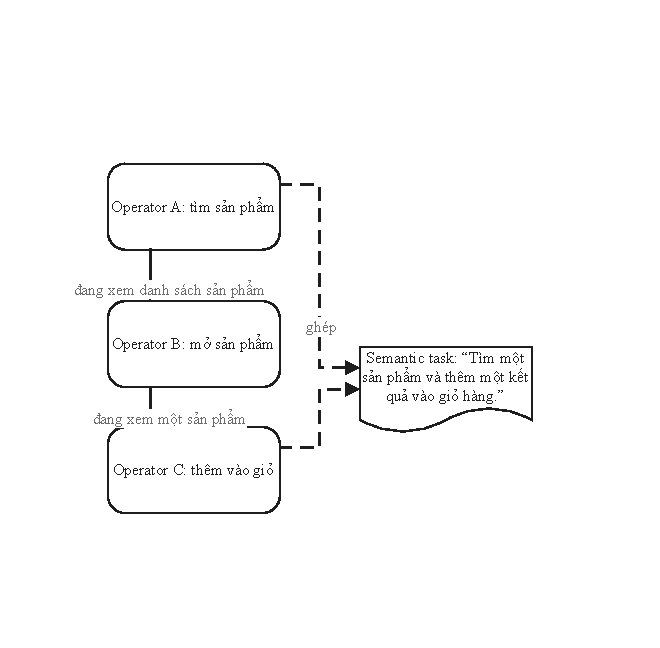
\includegraphics[width=0.78\textwidth]{Figures/fig_semantic.pdf}
\caption[Sinh semantic task bằng ghép chuỗi operator]{Sinh semantic task
bằng ghép chuỗi operator. Mỗi cạnh biểu diễn một trạng thái trung gian mà
effect của operator trước thỏa mãn precondition của operator kế tiếp. Các
chuỗi operator thu được tương ứng với những semantic task dài hạn, vượt ra
ngoài phạm vi của các task gắn với từng trang riêng lẻ.}
\label{fig:semantic}
\end{figure}

\subsection{Induction operator}

Sau khi một skill được thu nhận, thành phần \emph{inducer} sử dụng LLM để
suy ra \emph{precondition} và \emph{effect} của skill. Đầu vào gồm
\emph{SkillCard} cùng các quan sát ở đầu và cuối của một số trajectory đại
diện thuộc skill đó. Hai tập mệnh đề được sinh dưới dạng ngôn ngữ tự nhiên.

Prompt của bước này ràng buộc \emph{dạng} của mệnh đề chứ không chỉ nội dung,
và ràng buộc đó là điều kiện cần để việc ghép chuỗi về sau khả thi. Mỗi mệnh
đề phải mô tả một \emph{trạng thái trang} (``đang ở trang danh sách sản
phẩm'', ``trang giỏ hàng đang hiển thị'') chứ không phải sự hiện diện của một
phần tử đơn lẻ (``có một liên kết giỏ hàng trên trang''); phải có ít nhất một
precondition đặt tên cho trạng thái trang lúc vào và ít nhất một effect đặt
tên cho trạng thái trang lúc ra; và trạng thái lúc ra bắt buộc phải \emph{khác}
trạng thái lúc vào. Với một skill diễn ra gọn trong một trang, cách diễn đạt
được yêu cầu là giữ nguyên tên trang nhưng bổ nghĩa bằng điều mà skill vừa
thiết lập (``trang sửa sản phẩm \emph{đã có xác nhận lưu}''), tuyệt đối không
lùi về mức phần tử. Lý do của ràng buộc cuối này nằm ở chỗ chỉ một mệnh đề ở
mức trạng thái trang mới có cơ hội trùng với precondition của một skill khác;
lý do nó được viết thẳng vào prompt, thay vì được kỳ vọng, là kết quả của cổng
lọc ngay dưới đây (chi tiết ở Mục~\ref{sec:disc-operators}).

Nếu để LLM diễn đạt hoàn toàn tự do, các mệnh đề tương đương về ngữ nghĩa
thường được viết theo nhiều cách khác nhau, làm phân mảnh bộ từ vựng. Thực
nghiệm trên một lượt chạy cho thấy hiện tượng này xảy ra ngay cả khi sử dụng
sentence embedding để chuẩn hóa. Một cặp mệnh đề thực sự đồng nghĩa chỉ đạt
độ tương đồng 0{,}570, thấp hơn ngưỡng gộp 0{,}6, trong khi một cặp khác
nghĩa lại đạt 0{,}606; số liệu chi tiết được trình bày ở
Mục~\ref{sec:disc-operators}. Vì vậy, quá trình induction được thiết kế theo hướng \emph{vocabulary-aware}
(có nhận biết từ vựng đã dùng). Prompt cung cấp trước một tập các mệnh đề đã
có trong registry (sổ đăng ký mệnh đề, ưu tiên các mục được sử dụng nhiều và
mới nhất), đồng thời yêu cầu LLM tái sử dụng nguyên văn các mệnh đề tương
đương thay vì diễn đạt lại.

Operator sau khi sinh tiếp tục đi qua một bước kiểm tra
\emph{tautology} (mệnh đề hiển nhiên đúng). Các effect trùng hoàn toàn với
precondition sẽ bị loại bỏ

\[
\mathit{eff} \leftarrow \mathit{eff} \setminus \mathit{pre},
\]

và những skill không còn effect mới sau bước này sẽ không được nâng thành
operator. Mục đích của bước lọc là loại bỏ các operator không biểu diễn bất
kỳ thay đổi trạng thái nào, vì chúng không tạo ra cạnh mới trong đồ thị toán
tử và không thể tham gia vào quá trình ghép chuỗi.

Cổng lọc thứ hai kiểm tra một câu hỏi khác: mệnh đề vừa sinh ra có thực sự
đúng trên dữ liệu hay không. Khác với bước induction, vốn chỉ lấy hai
trajectory làm ngữ cảnh, bước này đối chiếu từng mệnh đề với trạng thái trang
trước và sau của \emph{mọi} thành viên trong cụm, rồi tính tỷ lệ số thành viên
mà mệnh đề đó thực sự đúng. Một effect được xác nhận trên dưới một nửa số
thành viên sẽ bị loại bỏ, và một operator không còn effect nào sau bước này sẽ
bị từ chối hoàn toàn. Ngưỡng này được đặt ở mức thận trọng, tương đương với
``chỉ loại những effect không đúng trên bất kỳ thành viên nào'', và nó có
nguyên nhân cụ thể: một lượt chạy trên Shopping Admin đã thu nhận một operator
với effect đạt độ chính xác 0{,}0, tức không đúng ở bất kỳ đâu, rồi vẫn lập kế
hoạch dựa trên nó.

Cần lưu ý rằng cổng này chỉ áp dụng cho effect. Các precondition cũng được
chấm điểm và ghi lại, nhưng không bao giờ bị loại bỏ, bởi việc gỡ đi một
precondition đáng ngờ sẽ khiến operator trở nên áp dụng được ở mọi nơi -- một
sai lầm nguy hiểm hơn nhiều so với việc quá thận trọng. Trong trường hợp cụm
không còn thành viên nào có dữ liệu trang để đối chiếu, cổng được bỏ qua thay
vì từ chối tất cả.

Một operator được đánh dấu là \emph{terminal} nếu ít nhất một trajectory thành
viên kết thúc tại trạng thái mục tiêu đã cấu hình, hoặc khi inducer xác định
skill đó tương ứng với việc hoàn thành mục tiêu.

\subsection{Chuẩn hóa mệnh đề}

Các mệnh đề sinh ra từ induction được chuẩn hóa thông qua
\emph{predicate registry} (sổ đăng ký mệnh đề). Thành phần này sử dụng cùng
cơ chế tính độ tương đồng cosine như thư viện skill, với ngưỡng mặc định
0{,}6 (Phụ lục~\ref{app:design-params}), nhưng không cho phép gộp các cụm đã
tồn tại, nhằm đảm bảo mỗi mã định danh sau khi cấp phát sẽ không thay đổi.

Đối với mỗi mệnh đề mới, hệ thống hoặc ánh xạ nó vào một cụm chuẩn hiện có và
kế thừa mã định danh của cụm đó, hoặc tạo một cụm mới nếu không tìm thấy
ứng viên phù hợp. Theo thời gian, registry xây dựng một tập predicate chung

\[
P=\{p_0,p_1,\ldots\},
\]

được chia sẻ bởi toàn bộ operator. Nhờ đó, việc so khớp giữa effect và
precondition chỉ còn là so sánh mã định danh thay vì so sánh trực tiếp chuỗi
văn bản, trong khi vẫn giữ được khả năng mở rộng bộ từ vựng thông qua LLM.

\subsection{Ghép chuỗi operator thành semantic task}

Đồ thị toán tử tạo một cạnh
$\omega_1 \rightarrow \omega_2$
nếu một effect của
$\omega_1$
khớp với một precondition của
$\omega_2$
sau bước chuẩn hóa. Trên đồ thị này, hệ thống sử dụng tìm kiếm theo chiều sâu
có chặn để liệt kê các đường đi đơn có độ dài từ hai trở lên. Các giới hạn về
độ dài chuỗi và số lượng đường đi được áp dụng nhằm tránh hiện tượng bùng nổ
tổ hợp khi đồ thị trở nên dày đặc.

Mỗi chuỗi operator thu được sẽ được chuyển thành một \emph{goal task} (tác vụ
mục tiêu). Nội
dung của task được tổng hợp từ mô tả của các skill trong chuỗi, còn điểm bắt
đầu lấy từ URL ghi nhận của operator đầu tiên. Chẳng hạn, nếu hệ thống đã
phát hiện hai skill ``tìm kiếm trong danh mục sản phẩm'' và ``thêm sản phẩm
đang hiển thị vào giỏ'', việc ghép hai operator tương ứng sẽ tạo ra một task
dạng \emph{``tìm một sản phẩm rồi thêm kết quả tìm được vào giỏ hàng''}.
Task này không được đề xuất từ bất kỳ trang riêng lẻ nào, mà được hình thành
từ quan hệ giữa các năng lực đã được kiểm chứng.

Các semantic task được thực thi theo chiến lược bảo thủ nhằm hạn chế lặp lại.
Trong mỗi lượt khám phá, mỗi chuỗi operator chỉ được thử tối đa một lần và
mỗi node chỉ sinh thêm một số lượng hữu hạn chuỗi mới. Thuật
toán~\ref{alg:semantic} mô tả toàn bộ quá trình này, từ việc liệt kê chuỗi
trên đồ thị toán tử cho tới cách chọn cơ chế kiểm chứng cho từng task.

\begin{algorithm}[H]
\caption{Sinh semantic task bằng ghép chuỗi operator}
\label{alg:semantic}
\begin{algorithmic}[1]
\Require đồ thị toán tử $G = (\Omega, E)$ với
$E = \{(\omega_1, \omega_2) : \mathit{eff}(\omega_1) \cap \mathit{pre}(\omega_2) \neq \emptyset\}$;
ngân sách $b$ chuỗi mới cho mỗi node; tập chuỗi đã thử trong lượt chạy $X$;
mục tiêu kết thúc $g_T$ (có thể không được cấu hình, ký hiệu $\bot$)
\Ensure danh sách semantic task kèm cơ chế kiểm chứng tương ứng
\State $P \gets \emptyset$
\For{mỗi $\omega \in \Omega$ theo thứ tự tất định}
  \State $\textsc{Dfs}([\omega])$
\EndFor
\State $T \gets \emptyset$
\For{mỗi chuỗi $p \in P$}
  \If{$|T| \ge b$} \textbf{break} \EndIf
  \If{$p \in X$} \textbf{continue} \Comment{mỗi chuỗi chỉ thử một lần trong một lượt chạy} \EndIf
  \State $X \gets X \cup \{p\}$
  \State $\mathit{instr} \gets$ URL khởi đầu ghi nhận của $p_1$, nối với mô tả các skill trong $p$ theo đúng thứ tự
  \If{$p_{|p|}$ được đánh dấu terminal \textbf{và} $g_T \neq \bot$}
    \State $\mathit{verify} \gets \textsc{Reached}(g_T)$ \Comment{kiểm chứng tất định}
  \Else
    \State $\mathit{verify} \gets$ kết luận của solver, judge kiểm tra lại ngay trong vòng lặp
  \EndIf
  \State $T \gets T \cup \{(\mathit{instr}, \mathit{verify}, |p|)\}$ \Comment{$|p|$ là độ khó}
\EndFor
\If{$T = \emptyset$ \textbf{và} $g_T \neq \bot$} \Comment{đồ thị còn quá thưa để ghép chuỗi}
  \State $p \gets \textsc{Plan}(G, \emptyset, g_T)$ \Comment{BFS tiến trên precondition/effect}
  \If{$p \neq \bot$}
    \State $T \gets \{(\text{tác vụ đạt mục tiêu kết thúc}, \textsc{Reached}(g_T), |p|)\}$
  \EndIf
\EndIf
\State \Return $T$
\Statex
\Function{Dfs}{$p$} \Comment{trả về \textbf{đúng} khi đã đủ số chuỗi cần liệt kê}
  \If{$|p| \ge \mathit{min\_len}$}
    \State $P \gets P \cup \{p\}$ \Comment{chuỗi con cũng là một task hợp lệ, ngắn hơn}
    \If{$|P| \ge \mathit{max\_paths}$} \State \Return \textbf{đúng} \EndIf
  \EndIf
  \If{$|p| \ge \mathit{max\_len}$} \State \Return \textbf{sai} \EndIf
  \For{mỗi $\omega'$ kế tiếp của $p_{|p|}$ theo thứ tự tất định, với $\omega' \notin p$}
    \If{$\textsc{Dfs}(p \text{ nối thêm } \omega')$} \State \Return \textbf{đúng} \EndIf
  \EndFor
  \State \Return \textbf{sai}
\EndFunction
\end{algorithmic}
\end{algorithm}

Việc đánh giá kết quả ưu tiên các tiêu chí tất định khi có thể. Nếu operator
cuối cùng là \emph{terminal} và website cung cấp điều kiện kết thúc có thể
kiểm tra bằng chương trình (chẳng hạn URL xác nhận đơn hàng), trạng thái
thành công sẽ được xác minh trực tiếp. Trong các trường hợp còn lại, episode
được đánh giá qua kết luận của solver và tiếp tục được một judge độc lập kiểm
tra lại \emph{ngay trong vòng lặp khám phá}: một phán quyết \textsc{Fail} sẽ
hạ episode xuống thất bại trước khi nó kịp đi vào bất kỳ khâu nào phía sau,
nên không episode nào được ghi nhận thành công chỉ dựa trên lời tự tuyên bố
của tác nhân (Mục~\ref{sec:method-data}, \ref{sec:disc-slm}).

Ở giai đoạn đầu khi đồ thị toán tử còn thưa và chưa hình thành được các chuỗi
hợp lệ, hệ thống tạm thời lập kế hoạch trực tiếp tới các trạng thái kết thúc
đã biết nếu có. Cơ chế này cho phép quá trình thu thập dữ liệu tiếp tục diễn
ra ngay cả trước khi đồ thị đủ phong phú để sinh semantic task.

\subsection{Seed năng lực website: nguồn mục tiêu từ trên xuống}
\label{sec:method-seed}

Cơ chế ghép chuỗi ở trên là một cơ chế \emph{từ dưới lên}: nó chỉ sinh được
task khi đồ thị toán tử đã có cạnh, mà cạnh lại chỉ hình thành khi hai
operator độc lập tình cờ phát biểu trùng một mệnh đề. Trong thực tế, điều
kiện này thưa hơn dự kiến rất nhiều (Mục~\ref{sec:disc-operators}), khiến
việc thu thập dữ liệu dài hạn bị treo vào tài sản khó xây dựng nhất của hệ
thống.

Vì vậy, hệ thống bổ sung một nguồn mục tiêu thứ hai, hoạt động \emph{từ trên
xuống} và không phụ thuộc đồ thị. Ở node đầu tiên của mỗi lượt khám phá,
thành phần \emph{site seeder} tóm tắt trang chủ thành một \emph{seed} gồm mô
tả website và một danh sách từ bốn tới tám năng lực mà website đó cho phép
người dùng thực hiện (chẳng hạn ``đặt hàng'', ``theo dõi trạng thái đơn
hàng'', ``quản lý sổ địa chỉ''). Mỗi năng lực trong seed trở thành một goal
task nhiều bước.

Prompt của seeder mang ba ràng buộc đáng chú ý, cả ba đều nhằm bảo đảm mục
tiêu sinh ra là thứ có thể chấm được. Thứ nhất, mỗi mục tiêu phải kết thúc ở
một trạng thái \emph{cụ thể và kiểm chứng được} từ trang kết quả, nên các hoạt
động mở như ``dạo xem danh mục điện tử'' bị cấm: đó là loại mục tiêu mà tuyên
bố hoàn thành gần như không tốn gì. Thứ hai, mọi giá trị đầu vào mà mục tiêu
cần phải hoặc được nêu thẳng trong mục tiêu, hoặc suy ra được từ trang (``sản
phẩm rẻ nhất'', ``đơn hàng gần nhất''); một mục tiêu để ngỏ giá trị cho tác
nhân tự nghĩ ra là mục tiêu mà tác nhân sẽ từ chối một cách hoàn toàn hợp lý.
Thứ ba, mọi năng lực phải bám vào những gì trang thật sự có, chứ không được
suy diễn ra các tính năng không nhìn thấy.

Ngân sách dành cho các mục tiêu này được phân bổ theo hai quy tắc. Một năng
lực có thể được thử lại tối đa ba lần trong một lượt chạy, mỗi lần từ một
\emph{loại} trang khác nhau (theo khuôn dạng URL), bởi cùng một mục tiêu theo
đuổi từ một điểm xuất phát khác thực sự là một quỹ đạo khác; ràng buộc theo
loại trang là thứ ngăn toàn bộ ngân sách bị tiêu hết trong vài node đầu tiên.
Ngược lại, một năng lực liên tiếp thất bại sẽ bị cho nghỉ sớm, và trường hợp
tác nhân tự tuyên bố bất khả thi thì bị cho nghỉ ngay lập tức: khi tác nhân đã
nhìn trang và kết luận rằng tính năng đó không tồn tại trên bản triển khai
này, kết luận ấy sẽ không đúng hơn ở trang thứ ba.

Seed đồng thời được đưa vào prompt của explorer làm ngữ cảnh, giúp các task
bậc thấp bám sát mục đích thật của website thay vì chỉ mô tả những gì trang
hiện tại hiển thị.

Hai nguồn này bổ trợ nhau và dùng chung ngân sách goal task của mỗi node:
ghép chuỗi cho ra các mục tiêu \emph{đã được kiểm chứng là khả thi} vì mọi
mắt xích đều là skill đã thu nhận, còn seed cho ra các mục tiêu \emph{đúng
mục đích của website} kể cả khi đồ thị còn trống. Tỷ trọng thực tế giữa hai
nguồn trong các lượt chạy thật được báo cáo ở Mục~\ref{sec:exp-data}.

So với các task được đề xuất độc lập trên từng trang, semantic task mang lại
hai lợi ích chính. Thứ nhất, chúng tạo ra các trajectory dài hơn, bao phủ
những chuỗi hành động nhiều bước thay vì chỉ các tương tác cục bộ. Thứ hai,
mỗi trajectory phản ánh việc phối hợp nhiều skill đã được kiểm chứng, từ đó
cung cấp các mẫu hành vi có cấu trúc phong phú hơn cho quá trình fine-tuning
mô hình ngôn ngữ nhỏ.

\section{Tinh lọc dữ liệu}
\label{sec:method-data}

Các episode thu được sau quá trình khám phá chưa thể sử dụng trực tiếp để
huấn luyện mô hình. Chúng tiếp tục trải qua ba giai đoạn xử lý nhằm kiểm soát
chất lượng và chuyển đổi thành tập dữ liệu fine-tuning, đồng thời duy trì
nguyên tắc \emph{prompt parity} trong toàn bộ pipeline
(Hình~\ref{fig:curation}).

\begin{figure}[htbp]
\centering
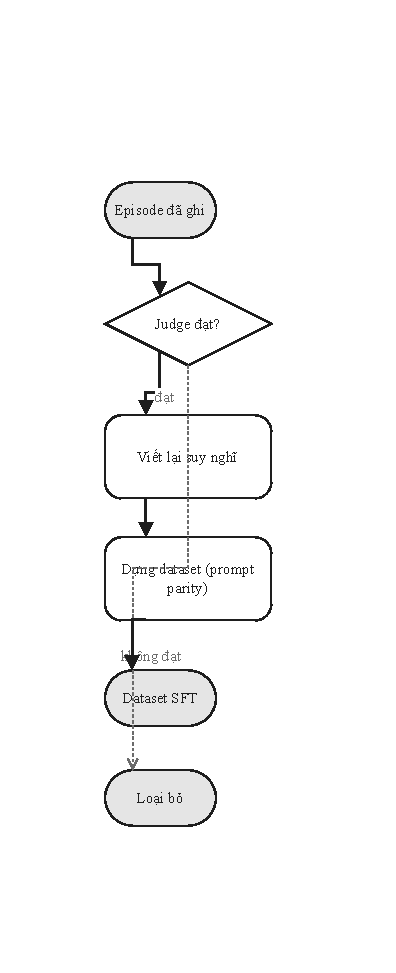
\includegraphics[width=0.50\textwidth]{Figures/fig_curation.pdf}
\caption[Pipeline tinh lọc dữ liệu]{Pipeline tinh lọc dữ liệu. Các episode
được một judge độc lập đánh giá lại, phần suy luận được chuẩn hóa, sau đó
được chuyển thành dữ liệu huấn luyện theo nguyên tắc prompt parity. Những
episode tự tuyên bố thành công nhưng không được judge xác nhận sẽ bị loại
khỏi tập dữ liệu.}
\label{fig:curation}
\end{figure}

\subsection{Chấm độc lập các thành công tự tuyên bố}

Một episode được solver kết luận là hoàn thành chưa đủ để xem là dữ liệu
đúng. Vì vậy, bước \emph{judge} sử dụng một LLM mạnh hơn để đánh giá lại tất
cả các episode tự tuyên bố thành công, theo cách tiếp cận dùng LLM làm bộ
chấm đã được kiểm chứng trong các nghiên cứu trước~\cite{zheng2023judge}.
Judge đối chiếu mục tiêu với trạng thái cuối của episode, bao gồm URL và nội
dung trang tại thời điểm kết thúc, rồi đưa ra một phán quyết độc lập. Những
phiên được xác minh bằng hàm kiểm tra tất định (\texttt{reached}) không đi qua
bước này, vì kết quả của chúng vốn đã đáng tin.

Điểm quan trọng là bước chấm này chạy \emph{ngay trong vòng lặp khám phá}, chứ
không phải sau khi lượt chạy kết thúc. Một phán quyết \textsc{Fail} hạ ngay
episode xuống thất bại \emph{trước khi} bất kỳ khâu nào phía sau nhìn thấy nó:
episode đó không được ghi là thành công, không đi vào khâu phát hiện kỹ năng,
và không được chọn cho lượt lấy mẫu không tiền tố. Vị trí của bước chấm là một
quyết định thiết kế có chủ đích: một phán quyết ngoại tuyến là phán quyết mà
lượt chạy \emph{không bao giờ hành động theo}, nên nó có thể sửa được tập dữ
liệu nhưng không sửa được những gì lượt chạy đã làm dựa trên kết luận sai.
Quyết định gọi judge cũng được đặt bên trong hàm giải một tác vụ thay vì ở các
nơi gọi hàm đó, để không một điểm gọi mới nào có thể vô tình bỏ qua nó. Hệ
thống vẫn giữ một kịch bản chấm ngoại tuyến độc lập, dùng chung prompt với bộ
chấm trực tuyến, để chấm lại các lượt chạy cũ thu thập trước khi cơ chế này
tồn tại.

Kết quả đánh giá của judge được lưu bổ sung bên cạnh kết luận ban đầu thay vì
ghi đè lên kết quả do solver tạo ra. Khi dựng dataset, hệ thống có thể lựa
chọn chỉ giữ lại các episode đã được judge xác nhận thành công, đồng thời
loại bỏ những episode chưa từng trải qua bước đánh giá này.

\subsection{Viết lại suy nghĩ (thought re-annotation)}

Chuỗi suy luận do solver sinh ra có chất lượng không đồng đều, trong khi đây
lại là tín hiệu mà mô hình fine-tune sẽ học theo. Do đó, mỗi bước suy luận
được viết lại theo một khuôn dạng thống nhất gồm bốn thành phần: (i) đánh giá
ngắn gọn về trạng thái hiện tại, (ii) phản tư nếu hành động trước đó không
đem lại tiến triển, (iii) \emph{subgoal} (mục tiêu con) của bước hiện tại và
(iv) ở bước kết thúc, một phép kiểm tra tường minh xem mục tiêu của task đã
được hoàn thành hay chưa.

Thành phần \emph{subgoal} được khôi phục bằng cách áp dụng lại chính thuật
toán phân đoạn trajectory sử dụng trong giai đoạn phát hiện skill. Quan trọng
hơn, thông tin này chỉ xuất hiện trong phần phản hồi của assistant
(\emph{assistant target}) và không được đưa vào prompt đầu vào. Thiết kế này
đảm bảo dữ liệu huấn luyện phản ánh đúng điều kiện suy luận thực tế, nơi mô
hình không được cung cấp trước subgoal của bước hiện tại.

\subsection{Dựng dataset với prompt parity}

Ở giai đoạn cuối, các episode được chuyển thành các mẫu instruction-tuning
(tinh chỉnh theo chỉ dẫn) theo nguyên tắc \emph{prompt parity}: cấu trúc
prompt sử dụng khi huấn luyện phải trùng khớp với prompt mà solver nhận được
trong quá trình suy luận.

Để đảm bảo tính nhất quán, system prompt được sử dụng trực tiếp từ solver thay
vì sao chép thủ công. Quan sát trang được cắt bằng đúng thủ tục tiền xử lý sử
dụng khi chạy agent, bao gồm cả các dấu hiệu cắt tường minh. Lịch sử tương
tác cũng được dựng theo đúng định dạng và chú thích kết quả mà agent quan sát
trong quá trình thực thi.

Những bước có hành động thực thi thất bại sẽ bị loại khỏi dữ liệu đích, vì
chúng là sai lầm chứ không phải cách khắc phục. Tuy nhiên chúng \emph{không}
bị xóa khỏi lịch sử của các bước sau: hành động đó đã thực sự xảy ra, và thông
báo lỗi mà nó sinh ra chính là thứ giải thích vì sao bước kế tiếp lại chọn một
hướng khác. Bỏ dòng lịch sử này đi thì mẫu huấn luyện của bước khắc phục sẽ
trông như được rút ra từ một trang chưa hề bị đụng tới, tức không còn khớp với
prompt mà mô hình thực sự nhìn thấy lúc suy luận.

Ngoài hai cổng đã nêu, khâu dựng dataset còn áp dụng ba bộ lọc ở mức episode.

\textbf{Cổng hành động hữu hiệu.} Một episode thuộc nhóm thay đổi trạng thái
hoặc điều hướng (\texttt{MOD}, \texttt{NAV}, \texttt{COMPOSITE}, hoặc một mục
tiêu ngữ nghĩa) sẽ bị loại nếu trong số các bước còn sống sau khi xuất ra
không có bất kỳ hành động nào thuộc nhóm có thể tác động lên trang. Nói cách
khác, một episode chỉ cuộn trang, di chuột hoặc chờ rồi tuyên bố hoàn thành là
một thành công giả, không phải một thành công ngắn. Cổng này bổ khuyết đúng
điểm mù của bộ chấm ngữ nghĩa: judge chỉ nhìn trạng thái cuối, mà trạng thái
cuối của một tác vụ ``sửa đổi'' không sửa gì thì trông hoàn toàn bình thường.
Nhóm \texttt{INFO} được miễn trừ, bởi trả lời ngay trên trang được đưa tới
chính là hình dạng đúng của nó.

\textbf{Loại bỏ báo cáo bất khả thi kiểu biện minh.} Chỉ những episode mà tác
nhân tự kết luận bất khả thi \emph{trong lúc} đang giải mới được giữ lại làm
mẫu huấn luyện. Những episode bị một chốt chặn dừng lại rồi mới phát ra
\texttt{report\_infeasible} ở lời gọi tổng kết đều bị loại, dựa trên lý do
dừng đã được lưu cùng episode (Mục~\ref{sec:method-solver}). Huấn luyện trên
nhóm sau là dạy mô hình bỏ cuộc, và hiệu ứng đó đo được: một tập dữ liệu chưa
lọc chứa 136 lần bỏ cuộc như vậy, chiếm 23\% số mẫu và tập trung vào đúng nhóm
tác vụ khó nhất, còn mô hình huấn luyện trên nó báo bất khả thi ở 39\% số tác
vụ Reddit khi đánh giá, đúng bằng tỷ lệ có trong dữ liệu.

\textbf{Loại bỏ hành động rời khỏi website.} Một hành động \texttt{goto} trỏ
tới một tên miền khác với trang hiện tại không bao giờ được dùng làm đích
huấn luyện. WebArena là tập hợp các bản sao tự triển khai của những website
thật, nên điều hướng sang chính website công khai mà bản sao đó mô phỏng sẽ
kết thúc phiên đánh giá với điểm 0. Khâu thu thập đã để lọt một hành động như
vậy, và mô hình sau fine-tune tái hiện đúng khuôn mẫu đó ở 10 trên 57 phiên
Reddit. Hành động này vẫn được giữ trong phần lịch sử, vì nó đã thực sự được
thực thi.

Mỗi mẫu dữ liệu đều mang theo mã trajectory, chỉ số bước và tổng số bước tương
ứng nhằm hỗ trợ quá trình gom lô theo trajectory. Cuối cùng, các mẫu được sắp
xếp theo mức độ khó tăng dần, với quy ước độ khó 1 cho quỹ đạo \texttt{LOCAL},
2 cho quỹ đạo \texttt{UNPREFIXED} và bằng độ dài chuỗi operator cho các mục
tiêu ngữ nghĩa, qua đó hình thành một curriculum cho quá trình fine-tuning
theo tinh thần của học theo chương trình (curriculum
learning)~\cite{bengio2009curriculum}.

\section{Fine-tune mô hình ngôn ngữ nhỏ}
\label{sec:method-sft}

Mô hình được sử dụng để fine-tune là Qwen3.5-9B~\cite{qwen2026qwen35}. Quá
trình huấn luyện áp dụng phương pháp
LoRA~\cite{hu2022lora} thông qua framework
LLaMA-Factory~\cite{zheng2024llamafactory}.

Việc chia tập huấn luyện và tập kiểm định được thực hiện theo đơn vị
\emph{tác vụ}, cụ thể là theo cặp (website, nội dung mục tiêu), chứ không theo
từng bước và cũng không theo từng quỹ đạo. Chia theo bước là sai hiển nhiên,
vì các bước trong cùng một episode quan hệ chặt với nhau. Nhưng chia theo quỹ
đạo cũng chưa đủ, và đây là điểm dễ bỏ sót: cơ chế lấy mẫu không tiền tố
(Mục~\ref{sec:method-unprefixed}) ghi lại mỗi tác vụ đã giải được \emph{hai}
lần, một lần từ chính trang của nó và một lần từ trang chủ, nên một mục tiêu
sở hữu hai quỹ đạo và một phép chia ở mức quỹ đạo sẽ đặt bản sao này vào tập
huấn luyện còn bản sao kia vào tập kiểm định. Đo trên chính tập dữ liệu của
khóa luận, cách chia đó làm rò rỉ 29 trên 56 quỹ đạo kiểm định, tương đương
một nửa số mẫu kiểm định: mô hình đã học đúng mục tiêu ấy, trên đúng website
ấy, tới đúng trang đích ấy. Hệ quả là giá trị \texttt{eval\_loss} trở nên lạc
quan và việc chọn checkpoint giữa các epoch dựa trên nó không còn đáng tin.

Hai xử lý phụ đi kèm phép chia. Thứ nhất, các bản lặp thừa bị loại bỏ: một mục
tiêu có đúng một quỹ đạo \texttt{LOCAL} và một quỹ đạo \texttt{UNPREFIXED} là
cặp đúng như thiết kế và được giữ nguyên, nhưng hai quỹ đạo \emph{cùng} mức độ
khó cho cùng một mục tiêu, vốn phát sinh khi một năng lực seed được đề xuất
lại ở node khác, chỉ giữ lại quỹ đạo dài nhất. Thứ hai, tập kiểm định được lấy
mẫu phân tầng theo từng website với cùng một tỷ lệ, thay vì lấy một lượt chung
trên toàn bộ dữ liệu; nếu không, website nào sở hữu các quỹ đạo dài nhất sẽ
chiếm phần lớn hạn mức kiểm định và \texttt{eval\_loss} sẽ chủ yếu phản ánh
riêng website đó.

Một điểm cần lưu ý khác là Qwen3.5-9B mặc định sinh ra các đoạn suy luận
tường minh (thinking), trong khi dữ liệu của khóa luận chỉ chứa các cặp
suy nghĩ--hành động đã được chuẩn hóa. Vì vậy, chat template được cấu hình
để vô hiệu hóa chế độ thinking trong cả quá trình huấn luyện lẫn suy luận,
đảm bảo định dạng đầu ra của mô hình nhất quán với dữ liệu huấn luyện.

Sau khi fine-tune, các trọng số LoRA được hợp nhất với mô hình gốc và triển
khai bằng vLLM~\cite{kwon2023vllm}. Cấu hình serving (phục vụ suy luận) tiếp
tục duy trì việc tắt chế độ thinking trên mọi yêu cầu. Nhờ đó, phân phối
prompt và đầu ra trong giai đoạn triển khai vẫn khớp với dữ liệu được sử dụng
khi huấn luyện, tương ứng với phía triển khai của nguyên tắc
\emph{prompt parity}.

\section{Ghi chú hiện thực hóa}
\label{sec:method-impl}

HSGE được hiện thực bằng Python. Bảng~\ref{tab:modules} trình bày sự tương
ứng giữa các giai đoạn của pipeline và các module trong hệ thống.

Một đặc điểm của kiến trúc là mỗi vai trò sử dụng LLM (site seeder, explorer,
solver, solver riêng cho tác vụ ngữ nghĩa, bộ lập kế hoạch subgoal, bộ cắt
đoạn, bộ trừu tượng hóa, bộ kiểm chứng, inducer, judge và bộ viết lại suy
luận) đều có thể cấu hình mô hình độc lập. Nhờ đó, các thành phần được gọi
thường xuyên có thể sử dụng những mô hình chi phí thấp hơn, trong khi các mô
hình mạnh hơn được dành cho những bước yêu cầu chất lượng cao như giải tác vụ
ngữ nghĩa, operator induction và judge. Hai vai trò tương tác trực tiếp với
trang, tức explorer và solver, còn có thể được bật chế độ thị giác: khi đó
prompt được đính kèm ảnh chụp màn hình, tùy chọn phủ thêm lớp đánh dấu
Set-of-Marks vẽ khung bao quanh các phần tử theo đúng mã định danh xuất hiện
trong cây trợ năng. Vì một lời gọi có đính ảnh đôi khi bị phía nhà cung cấp
trả về rỗng, cả hai vai trò đều thử lại một lần ở chế độ thuần văn bản trước
khi chấp nhận thất bại.

Việc đăng nhập vào các website có xác thực được thực hiện một lần và lưu lại
trạng thái phiên; các lượt chạy sau nạp lại trạng thái đã lưu và bắt đầu trong
tình trạng đã đăng nhập, thay vì lặp lại luồng đăng nhập. Đây cũng là lý do
mọi tác vụ liên quan tới tài khoản đều bị cấm ở khâu đề xuất
(Mục~\ref{sec:method-lowlevel}): tài khoản là tài nguyên dùng chung giữa các
lượt chạy, và một thao tác đăng xuất hay đổi mật khẩu có thể khóa toàn bộ các
lượt chạy sau ra ngoài.

Toàn bộ pipeline cũng được thiết kế theo hướng tách biệt giữa thuật toán và
backend (lớp thực thi bên dưới). Hệ thống hỗ trợ cả backend thật và các
backend mô phỏng tất định (LLM theo kịch bản, embedding giả lập và website mô
phỏng), trong đó backend thật chỉ là một hiện thực khác của cùng giao diện. Thiết kế này
cho phép kiểm thử đơn vị các thành phần cốt lõi bằng các điều kiện kiểm tra
xác định, đồng thời giảm sự phụ thuộc vào chi phí API cũng như trạng thái
hoạt động của website trong quá trình phát triển.

Để hỗ trợ khả năng khôi phục sau khi gián đoạn, các sản phẩm trung gian như
skill, operator, đồ thị toán tử, kết quả khám phá của từng node và nhật ký sự
kiện đều được lưu sau mỗi node khám phá. Ngoài các sản phẩm ở dạng đọc được,
hệ thống còn ghi một điểm kiểm tra (checkpoint) nhị phân chứa toàn bộ trạng
thái vòng lặp, gồm hàng đợi frontier, tập đã thăm, các bộ đếm và toàn bộ đối
tượng của khâu phát hiện. Điểm kiểm tra được ghi theo cơ chế thay thế nguyên
tử sau mỗi node, nên một lần dừng đột ngột chỉ mất đúng node đang xử lý dở, và
lượt chạy có thể nối tiếp từ đúng chỗ đã dừng thay vì bắt đầu lại. Các đối
tượng backend (khách LLM, bộ nhúng) không tuần tự hóa được nên được tháo ra
trước khi ghi và gắn lại sau khi nạp.

Ngoài ra, mọi thao tác trình duyệt trong vòng lặp đều được thiết kế theo hướng
hỏng mềm (fail-soft): một node không tải được sẽ được ghi log, ghi nhận kèm
lỗi rồi bỏ qua, thay vì làm dừng cả lượt chạy nhiều giờ. Ngược lại, một ngoại
lệ thật sự bất ngờ ở bất kỳ nơi nào khác vẫn được để cho lan lên và làm dừng
lượt chạy một cách ồn ào, sau khi đã ghi lại trạng thái lỗi.

\begin{table}[H]
\centering
\caption[Các giai đoạn pipeline và module hiện thực]{Các giai đoạn pipeline
và module hiện thực tương ứng.}
\label{tab:modules}
\begin{tabular}{@{}L{5.2cm} L{8.0cm}@{}}
\toprule
\textbf{Giai đoạn} & \textbf{Module} \\
\midrule
Vòng khám phá, frontier &
\texttt{webarena/runtime},
\texttt{webarena/browser} \\

Đề xuất và giải task &
\texttt{webarena/agents} \\

URL độc lập máy chủ &
\texttt{webarena/urls} \\

Đăng nhập và phiên đã lưu &
\texttt{webarena/auth} \\

Cắt đoạn &
\texttt{segmentation},
\texttt{discovery} \\

Gom cụm, thư viện skill &
\texttt{clustering},
\texttt{abstraction},
\texttt{library} \\

Operator và lập kế hoạch &
\texttt{operators},
\texttt{operator\_induction},
\texttt{predicate\_registry} \\

Chấm lại episode (trực tuyến và ngoại tuyến) &
\texttt{webarena/verify},
\texttt{judge\_episodes} \\

Tinh lọc dữ liệu &
\texttt{reannotate\_thoughts},
\texttt{build\_sft\_dataset} \\

Chia train/val, gộp nhiều website &
\texttt{training/prepare\_dataset},
\texttt{training/merge\_datasets} \\

Huấn luyện và serving &
cấu hình LLaMA-Factory, script vLLM \\
\bottomrule
\end{tabular}
\end{table}

\vspace{1em}
\noindent
Sau khi trình bày toàn bộ phương pháp, chương tiếp theo đánh giá hiệu quả của
pipeline trên môi trường WebArena. Nội dung thực nghiệm tập trung vào hai câu
hỏi: pipeline thu thập được bao nhiêu dữ liệu huấn luyện từ website thực tế,
và việc fine-tune trên tập dữ liệu này có cải thiện khả năng thực hiện task
của mô hình trên benchmark WebArena hay không.
